\chapter{Technical Background on Optimal Transport}
\label{chap:1}

% \localtableofcontents
\renewcommand{\contentsname}{Contents}
\localtableofcontents*
\chaptermark{\textbf{Technical Background on Optimal Transport}}

\hfill \break
In this chapter, we provide relevant technical background to three problems:
balanced optimal transport (OT), unbalanced OT and Gromov-Wasserstein distance.
The general structure for each topic includes the motivation, the theoritical and numerical aspects.
In particular, we focus on the numerics, which are not usually discussed in the OT literature,.
By contrast, we only briefly present the theory since it has already been well-studied and
can be found in many prior works, which will be precised during the discussion of each topic.

We start with the balanced OT, which compares probability measures
whose supports live in the same underlying space. Then, we study two important extensions
of this problem. The first one is based on the relaxation of the hard marginal constraints,
which results in the unbalanced OT. The second generalization
considers the situation where the supports of the probability measures lie in
incomparable ground spaces. This leads to the Gromov-Wasserstein distance,
whose origin comes from the Gromov-Hausdorff distance adapted to the Wasserstein distance.

\raggedbottom

%%%%%%%%%%%%%%%%%%%%%%%%%%%%%%%%%%%%%%%%%
\section{From Wasserstein distance}

\subsection{Balanced Optimal Transport}

We present two viewpoints on the motivation of the OT problem:
the Monge problem serves as the historical starting point and
the Hausdorff distance later provides the intuition to the Gromov-Wasserstein distance.
Then, we introduce some important theoritical properties of the Wasserstein distance,
which are widely used in machine learning applications.
Finally, we discuss in details the algorithmic and practical aspects of the
entropic approximation of the OT distance.

\subsubsection{Motivation} \label{subsec:ot_motiv}

\paragraph{Relation with Monge's problem}
The original OT problem was first formulated by \citep{Monge81}. From a mathematical viewpoint,
it aims to transport all the mass from one probability distribution to the other, so that
the displacement cost is minimized. Typically, this cost is measured by a distance function which
takes supports of the probability measures as inputs. Transporting from one probability measure
$\mu$ to the other one $\nu$ is equivalent to finding a map $T$ such that $\nu = T_{\# \nu}$.
\begin{definition}[Push-forward measure]
  Let $X, Y$ be two measurable spaces. Given a probability measure $\mu$ on $X$ and a
  measurable map $T: X \to Y$, we call $T_{\# \mu} \in \cP(Y)$ the \textbf{push-forward} measure of
  $\mu$ by $T$, defined by $T_{\# \mu}(E) = \mu(T^{-1}(E))$, for every $E \subset Y$. Equivalently,
  for every measurable bounded function $\varphi: Y \to \bbR$, we have
  $\int_Y \varphi \; d T_{\# \mu} = \int_X \varphi \circ T \; d\mu$.
  We also say $T$ is a \textbf{transport map} from $\mu$ to $\nu$.
\end{definition}
\begin{definition}[Monge's problem]
  Let $X, Y$ be two metric spaces. Given two probability measures $\mu \in \cP(X), \nu \in \cP(Y)$
  and a measurable cost function $c: X \times Y \to \bbR \cup \{\infty\}$,
  we define the Monge's problem as
  \begin{align}
    \text{MOT}(\mu, \nu) = \inf_{T \in \cT(\mu, \nu)} \int_X c(x, T(x)) \; d\mu(x),
  \end{align}
\end{definition}
where $\cT(\mu, \nu) := \{T: X \to Y \text{ measurable such that } T_{\# \mu}= \nu \}$ is the
set of transport maps from $\mu$ to $\nu$.
Despite the natural interpretation, the Monge's formulation has some major drawbacks.
First, its objective function is nonconvex,
thus brings much difficulty to the theoretical analysis and numerical optimization.
Second, the transport map may not exist.
For example, if the supports of $\mu$ and $\nu$ are finite such that $|\supp(\mu)| > |\supp(\nu)|$,
then the set $\cT(\mu, \nu)$ is empty because any transport map must be surjective.
Even when it exists, there is no guarantee that the infimum can be attained.
Last but not least, the Monge's problem is asymmetric,
in the sense that $\text{MOT}(\mu, \nu) \neq \text{MOT}(\nu, \mu)$.

Instead of enforcing one-to-one relation, we can allow one-to-many alignment,
meaning that the mass transported by a source point can be splitted to various target points.
Formally, we consider the set of admissible couplings (or transport plans) defined as
\begin{align}
  U(\mu, \nu) := \{ \pi \in \cP(X \times Y): \pi_{\# 1} = \mu, \pi_{\# 2} = \nu \},
\end{align}
where $\pi_{\# 1} = \int_Y d \pi(\cdot, y)$ and $\pi_{\# 2} = \int_X d\pi(x, \cdot)$
are the marginal distributions of the measure $\pi$. Clearly, $\cT(\mu, \nu) \subset U(\mu, \nu)$,
since for any transport map $T$ (if exists), we have $(\id, T)_{\# \mu} \in U(\mu, \nu)$. Now,
we are ready to define the relaxation of the Monge problem,
known as the \textit{Kantorovich's problem} \citep{Kanto42}.
\begin{definition}[Kantorovich's problem]
  Let $X, Y$ be two compact metric spaces. Given $\mu \in \cP(X), \nu \in \cP(Y)$
  and $c: X \times Y \to \bbR \cup \{\infty\}$, the Kantorovich's problem is
  the following optimization problem
  \begin{align}
    \label{eq:kanto_prob}
    \ot(\mu, \nu) = \inf_{\pi \in U(\mu, \nu)} \int_{X \times Y} c(x, y) \; d\pi(x, y).
  \end{align}
\end{definition}
Throughout this thesis, we refer Problem \eqref{eq:kanto_prob} to as the OT problem.
When $c(x, y) = d^p(x, y)$, for $p \geq 1$ and $d$ is the (common) metric on the metric spaces
$X$ and $Y$, we obtain the famous Wasserstein distance of order $p$ \citep{Villani03}.
\begin{align}
  W^p_p(\mu, \nu) = \inf_{\pi \in U(\mu, \nu)} \int_{X \times Y} d^p(x, y) \; d\pi(x, y).
\end{align}
Since $\cT(\mu, \nu) \subset U(\mu, \nu)$, we have $\text{MOT}(\mu, \nu) \geq \ot(\mu, \nu)$.
Equality may hold, for example in the cases of the celebrated Brenier's theorem \citep{Brenier87}
for continuous measures, and of the Birkhoff-von-Neumann theorem \citep{Birkhoff46}
for the discrete ones.

\paragraph{Relation with Hausdorff distance}
So far, we have seen the derivation of the OT from the Monge's problem.
Now, we present another approach based on the Hausdorff distance.
Most materials are taken from \citep{Memoli11}.

Given a compact metric space $(Z, d)$, we denote $\cC(Z)$ the collection of all compact subsets of
$Z$. The Hausdorff distance between $X, Y \in \cC(Z)$ is defined as
\begin{align}
    d_{H}^{(Z, d)}(X,Y) := \max \left( \sup_{x \in X} d(x,Y), \sup_{y \in Y} d(y,X) \right),
\end{align}
where the distance between a point to a subset of a metric space is defined by
$d(x,Y) := \inf_{y \in Y} d(x,y)$.
It is known that $d_{H}^{(Z, d)}$ is a proper metric on $\cC(Z)$ (see for example,
Proposition 7.3.3 in \citep{Burago01}).
% Equivalently, we have
% \begin{align}
%   d_{H}^{(Z, d)}(X,Y) = \sup_{z \in K} \left| d(z,Y) - d(z,X) \right|,
% \end{align}
% for any $K \in \cC(Z)$ such that $X \cup Y \subset K$ (see for example, \citep{Aamari22}).
% Now, we consider a different formulation of the Hausdorff distance.
%%%%%%%%%%%%%%%%%%%%%%%%%%%%%%%%%%%
\begin{definition}[Correspondance]
Given two non-empty sets $X$ and $Y$,
a subset $R \subset X \times Y$ is a correspondance between $X$ and $Y$ if and only if
\begin{itemize}
    \item[$\bullet$] For every $x \in X$, there exists $y \in Y$ such that $(x,y) \in R$.
    \item[$\bullet$] For every $y \in Y$, there exists $x \in X$ such that $(x,y) \in R$.
\end{itemize}
\end{definition}
%%%%%%%%%%%%%%%%%%%%%%%%%%%%%%%%%%%%%%%%%%%%%%%%%%%%%%%%%%%%%%%%%%%%%%
An example of correspondance is illustrated in \Cref{fig:correspondance}.
When $X$ and $Y$ are finite with cardinals $m$ and $n$, respectively,
then all correspondances can be constructed as follows:
choose a matrix $M \in \{0,1 \}^{m \times n}$ such that every row and column
contains at least a value $1$, then the correspondance can be defined as
$R:= \{(x_i, y_j) \in X \times Y: M_{ij} = 1 \}$. In particular, if $X$ and $Y$ are disjoint,
then $R$ corresponds to a bipartite graph in which every edge has uniform weight of one.
In this case, there is an intimate relation between the correspondance
and the transportation plan in OT
\footnote{More discussion on the bipartite-graph viewpoint of OT can be found in
Chapter 8 in \citep{Brualdi06} or Chapter 3.4 in \citep{Peyre19}.}.
First, both describe the alignments between $X$ and $Y$.
Second, the transport plan can also be seen as a flow in a bipartite graph,
where the source nodes must be connected to all target nodes via weighted edges.
\begin{figure}[t]
  \centering
  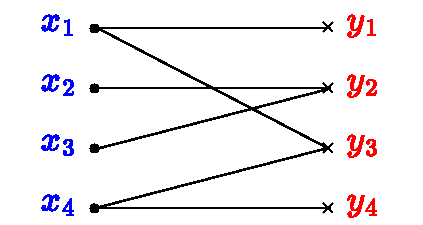
\includegraphics[width=0.35\textwidth,keepaspectratio]{Chapitre1/figures/correspondance.pdf}
  \caption{Example of correspondance $R$ between two sets $X = \{x_1, x_2, x_3, x_4\}$ and
  $Y = \{y_1, y_2, y_3, y_4 \}$. Here,
  $R = \{(x_1, y_1), (x_1, y_3), (x_2, y_2), (x_3, y_2), (x_4, y_3), (x_4, y_4) \}$.}
  \label{fig:correspondance}
\end{figure}
Denote $\mathcal R(X,Y)$ the collection of all correspondances between $X$ and $Y$,
then by Proposition 2.1 in \citep{Memoli11}, we have
\begin{align} \label{haus_corres}
  d_{H}^{(Z, d)}(X,Y) = \inf_{R \in  \mathcal R(X,Y)} \sup_{(x,y) \in R} d(x,y)
  = \inf_{R \in \mathcal R(X,Y)} \vert\vert d \vert\vert_{L^{\infty}(R)}.
\end{align}
Suppose that we equip each compact subset in $\cC(Z)$ with a Borel probability measure and consider
the collection of such "weighted spaces"
$\cC_w(Z) := \{(X,\mu_X): \text{supp}(\mu_X) = X \text{ and } X \in \cC(Z) \}$.
Given the similarity discussed above,
one can replace the correspondance by the admissible coupling and obtain the Wasserstein distance
\begin{align}
  W_{Z, \infty}\big((X,\mu_X), (Y,\mu_Y) \big) :=
  \inf_{\pi \in U(\mu_X, \mu_Y)} \sup_{(x,y) \in R(\pi)} d(x,y)
  = \inf_{\pi \in U(\mu_X, \mu_Y)} \vert\vert d \vert\vert_{L^{\infty}(R(\pi))},
\end{align}
where $R(\pi) := \text{supp}(\pi)$ the support of the measure $\pi$. Note that,
by Lemma 2.2 in \citep{Memoli11}, for any $\pi \in U(\mu_X, \mu_Y)$, we have
$R(\pi) \in  \mathcal R(\text{supp}(\mu_X), \text{supp}(\mu_Y))$, thus
$d_{H}^{(Z, d)} \leq W_{Z, \infty}$. By replacing the supremum norm with the $L^p$-norm,
we recover the $p$-Wasserstein distance
\begin{align}
    W_{Z, p}\big( (X,\mu_X), (Y,\mu_Y) \big)
    = \inf_{\pi \in U(\mu_X, \mu_Y)} \vert\vert d \vert\vert_{L^p(X \times Y, \pi)}.
\end{align}
To conclude, Diagram \ref{fig:wass_motiv} summarizes
the process of transforming the Hausdorff distance into the $p$-Wasserstein distance,
when the compact metric space is equipped with a probability measure.
As we will see in \Cref{sec:gw}, this process is particularly useful
when extending to the setting of metric measure space.
\begin{figure}[ht]
  \centering
  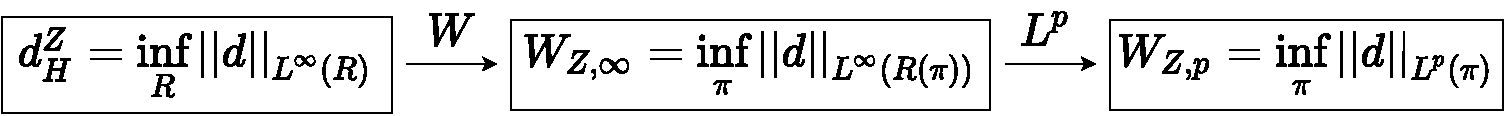
\includegraphics[width=0.85\textwidth,keepaspectratio]{Chapitre1/figures/wass_motiv.pdf}
  \caption{"W" indicates the \textit{Wassersteinization} process: replacing the optimization over the correspondances by over the admissible couplings.
  "$L^p$" indicates the \textit{$L^p$-ization} process: replacing the supremum norm by the $L^p$-norm.}
  \label{fig:wass_motiv}
\end{figure}
\subsubsection{Theory}
Since the seminal work of Kantorovich \citep{Kanto42},
the theory of OT has been profoundly developped in the last decades.
Different theoretical aspects with different level of generality
(from compact metric space to Polish space) are covered in various excellent references,
to name just a few, \citep{Villani03,Villani08,Fillipo15,Ambrosio05}. This list is
by no means exhaustive or representative. In this thesis, we only present a few
basic and useful properties of OT, which have much impact in machine learning.

\paragraph{Existence of solution, metric and weak convergence properties}
The existence of minimizer of the Kantorovich problem is guaranteed,
for example when the cost is lower semi-continuous and bounded below
(Theorem 4.1 in \citep{Villani08}). Note that,
apart from the classic choice of cost function $c = d^p$ as in the Wasserstein distance,
there are other alternatives, for example, the Bregman divergence \citep{Guo21},
or even the Wasserstein distance \citep{Huizing22}.

The Wasserstein distance defines a metric
on the space of probability measures with finite moments of order $p \geq 1$
(Theorem 7.3 in \citep{Villani03}) and characterizes the weak convergence: for any $p \geq 1$,
we have $\mu_n \rightharpoonup \mu$ if and only if $W_p(\mu_n, \mu) \to 0$
(Theorem 7.12 in \citep{Villani03}).
This topological property also holds for the integral probability metric \citep{Muller97},
but not for other popular statistical divergences, namely the Kullback-Leibler divergence,
total variation, Hellinger distance
\footnote{More detailed comparison amongst divergences can be found in \citep{Gibbs02}.}.

\paragraph{Duality theory}
Given the convexity of the OT problem, another very powerful property
is the duality theorem, which asserts that the strong duality holds. More precisely,
if $X, Y$ are compact metric spaces and the cost $c$ is continuous, then by Theorem 1.46
in \citep{Fillipo15}, one has
\begin{align}
  \ot(\mu, \nu) = \sup_{\substack{(f, g) \in \cC_b(X) \times \cC_b(Y) \\ f \oplus g \leq c}} \;
  \int_X f d\mu + \int_Y g d\nu,
\end{align}
where $\cC_b(X), \cC_b(Y)$ denote the space of bounded continuous functions on $X, Y$, respectively.
Strong duality still holds in a much more general setting (see Theorem 5.10 in \citep{Villani08}).
The theory of duality plays a crucial role, not only in theoritical study, but also
in practical applications. In particular, it is at the heart of some exact solvers
for the discrete OT problem (see Section 3 in \citep{Peyre19}).
In the case of Wasserstein distance, the duality theory allows to deduce other reformulations
of the primal problem, which have recently attracted much interest in machine learning.
We now discuss two particular important applications.

\paragraph{$2$-Wasserstein distance}
Under mild assumptions on the probability measures, thanks to the duality and
Brenier's theorems \citep{Brenier87}, Theorem 2.9 in \citep{Villani03} states that
the $2$-Wasserstein distance can be rewritten as the optimization of convex functions.
This result has been used to estimate the Wasserstein distance
\citep{Chartrand09,Taghvaei19,Korotin19,Makkuva20},
where the functional is parametrized by an input convex neural network \citep{Amos17}.

\paragraph{$1$-Wasserstein distance}
An important application of the duality theory is the $1$-Wasserstein distance
(also known as \textit{Earth mover's distance}). Its dual problem
\footnote{Also known as the \textit{Kantorovich-Rubinstein duality}, see Remark 6.5
in \citep{Villani08}. More discussion on the $1$-Wasserstein distance can be found
in Chapter 6 in \citep{Peyre19}.}
is a reformulation of the primal problem as the maximization over all $1$-Lipschitz functionals,
which can be parametrized by neural networks.
In practice, the the $1$-Wasserstein distance has been successfully used
in the training of generative adversarial networks (GAN) \citep{Goodfellow14},
thanks to the seminal work of \citep{Arjovsky17} on Wasserstein GAN (WGAN).
There have been various extensions and improvements of WGAN, for example
smoothed WGAN \citep{Sanjabi18}, WGAN-GP \citep{Gulrajani17}, WGAN-LP \citep{Petzka18},
Sobolev-GAN \citep{Mroueh17}. It is also the motivation for other OT-based GAN methods, namely
Sinkhorn divergence-GAN \citep{Genevay18a}, OT-GAN \citep{Salimans18}.
Interestingly, WGAN also finds its connections with the Minkowski and Alexandrov problems
in convex geometry \citep{Lei19}, and with the soft-margin formulation of
Support Vector Machine \citep{Jolicoeur19}.

\subsubsection{Approximation and algorithm}
In discrete setting, the OT formulation is a linear program.
An example of exact solver \footnote{See also Chapter 3 in \citep{Peyre19}
for a more detailed discussion on classic algorithms and Section 2.1 in \citep{Pele09}
for an overview on computational complexity.}
is the interior point method \citep{Orlin88}. It requires the complexity of $O(n^3 \log n)$,
which is computationally prohibitive in many applications.
There exist some approaches to overcome this limitation. For example, the mini-batch approach
\citep{Sommerfeld19,Fatras20} considers multiple resamplings of the data and
uses the average of distances computed in the mini-batches as an estimation of the true OT distance.
The "sliced" method \citep{Rabin12,Bonneel15} develops an alternative metric
called \textit{Sliced Wasserstein distance}.
It relies on the fact that computing the $1$-D Wasserstein distance boils down to sorting the
point values, which only requires the complexity of $O(n \log n)$.
Using the framework from statistical physics, \citep{Koehl19}
approximate the OT distance by the free energy evaluated at sufficiently small temperature.
From a more mathematical viewpoint, this idea is based on the interesting relation
between the minimum and the logsumexp operation, where informally, one has that:
$\min f(x) = \lim_{\beta \to 0^+} -\frac{1}{\beta} \int e^{-\beta f(x)} dx$.

\paragraph{Entropic OT problem}
In this thesis, we focus on the line of works on the discrete entropic approximation
\footnote{For a mathematical introduction in the general setting,
interested readers may consult the lecture note of \citep{Nutz22}.} defined by:
for $\varepsilon > 0$,
\begin{align}
  \label{eq:primal_ot}
  \ot_{\varepsilon}(\mu, \nu) = \inf_{P \in U(\mu, \nu)} \langle C, P \rangle +
  \varepsilon \; \kl(P | \mu \otimes \nu).
\end{align}
In the OT literature, the entropic regularization can sometimes be referred to the case where
the regularizer is the negative entropy defined by $H(P) = \sum_{i,j} P_{ij} (\log P_{ij} - 1)$.
However, since $\kl(P | \mu \otimes \nu) = H(P) - H(\mu) - H(\nu)$, for any $P \in U(\mu, \nu)$,
the two regularized problems are equivalent, up to a constant.
Interestingly, the entropic OT is an even older problem than the unregularized one.
It was already studied in the early 30's by \citep{Schrodinger32},
under the name \textit{static Schrodinger bridge problem}.
The entropic OT problem has attracted much attention to the
machine learning community thanks to the seminal work of \citep{Cuturi13}.

Note that, the entropic regularization introduces bias,
in the sense that $\ot_{\varepsilon}(\mu, \mu) \neq 0$, for any $\varepsilon > 0$.
This issue can be easily overcome by considering the Sinkhorn divergence
\footnote{This divergence is implemented very efficiently in the Geomloss package \citep{Feydy19}.}
\citep{Ramdas17,Feydy19} defined by
\begin{align}
  \text{SD}_{\varepsilon}(\mu, \nu) = \ot_{\varepsilon}(\mu, \nu)
  - \frac{1}{2} \left[ \ot_{\varepsilon}(\mu, \mu) + \ot_{\varepsilon}(\nu, \nu) \right].
\end{align}
Not only being unbiased, the Sinkhorn divergence also enjoys favorable topological, statistical
and interpolation properties \citep{Feydy19,Genevay19}. In particular,
if the cost is the squared $l_2$-norm, then it is a good proxy
for the squared $2$-Wasserstein distance. More precisely, under mild conditions on $\mu$ and $\nu$,
one has that $| \text{SD}_{\varepsilon}(\mu, \nu) - W_2^2(\mu, \nu) | = O(\varepsilon^2)$
\citep{Chizat20}.

\paragraph{Properties} The entropic OT has many interesting properties. First, it is a
good and scalable approximation of OT distance,
where the approximation error can be quantified in some settings \citep{Genevay19,Luise18}.
Moreover, the convergence behaviors of minimum and minimizer are also well understood
\citep{Leonard12,Carlier17} and the convergence rate exists in some practical situations
\citep{Genevay19,Cominetti94,Weed18}.
Second, since entropic OT is a convex problem, strong duality holds and one has that
\begin{align}
  \label{eq:dual_ot}
  \ot_{\varepsilon}(\mu, \nu) = \sup_{\substack{f \in \bbR^m \\ g \in \bbR^n}}
  \langle f, \mu \rangle + \langle g, \nu \rangle
  - \varepsilon \; \left\langle \exp \left( \frac{f \oplus g - C}{\varepsilon} \right), \mu \otimes \nu \right\rangle.
\end{align}
Arguably, this is the most important premise in the study of the entropic approximation, which
allows to develop and analyze many Sinkhorn-based algorithms (see \Cref{para:summary} for discussion).
In particular, \citep{Genevay19} use the dual problem to show that entropic OT
has better sample complexity than unregularized OT,
though it fixes the bottleneck in the sample size by introducing a new one in the regularization.
This issue can be mitigated, for example when the probability measures are sub-Gaussian \citep{Mena19}.
Entropic OT is also known for its joint convexity, smoothness with respect to
the inputs \citep{Luise18} and metric property \citep{Sanjabi18}.

\paragraph{Algorithm} To solve the dual problem \eqref{eq:dual_ot},
we are interested in the deterministic approach, where the most popular solver
is the Sinkhorn algorithm \citep{Sinkhorn67}
\footnote{Also known as \textit{matrix scaling algorithm}.
For the historical perspective, see Remark 4.5 in \citep{Peyre19}.}.
Denote $K = e^{-C / \varepsilon}$ the kernel matrix. Then,
from the first-order optimality conditions of the dual problem, the iterates read
\begin{align}
  u^{(t+1)} = \frac{\mu}{Kv^{(t)}} \text{ and } v^{(t+1)} = \frac{\nu}{K^T u^{(t+1)}}.
\end{align}
This algorithm is very easy to implement and available in the Python Optimal Transport
\citep{Flamary21} and OTT-JAX \citep{Cuturi22} packages.
It is well known that it converges globally to the optimal dual vectors of the dual problem
\citep{Sinkhorn67}, at a linear rate in variation semi-norm \citep{Franklin89}.
The OT plan then can be retrieved from the optimal solution $(u, v)$ by
$P = (\mu \otimes \nu) \odot (u \otimes v) \odot K$, where $\odot$ is the element-wise multiplication.

% Note that, as Sinkhorn algorithm is nothing but a coordinate ascent algorithm,
% \footnote{Note that the "one-at-a-time" scheme must be used
% (\ie $u^{(t+1)}$ is used in the calculation of $v^{(t+1)}$), whereas the "all-at-once" scheme
% (\ie $u^{(t)}$ is used in the calculation of $v^{(t+1)}$) does not necessarily guarantee the convergence.
% See, for example \url{https://www.stat.cmu.edu/~ryantibs/convexopt-F16/scribes/coord-desc-scribed.pdf}.}

\paragraph{Discussion on Sinkhorn algorithm}
The Sinkhorn algorithm has two key advantages. First, since the iterates only require
vector-matrix multiplication, they can be seamlessly parallerized.
One can further speed up the computation by exploiting the structure of the kernel matrix
(see Section 4.3 in \citep{Peyre19}). Second, it is enough to store only the dual vectors
(which cost $O(n)$ in memory) because the OT plan (which costs $O(n^2)$ in memory)
can be easily queried on demand.

However, the smaller the regularization, the more it hurts the Sinkhorn algorithm.
First, if the number of iterations is not sufficiently large,
the algorithm may fail to converge and the resulting transport plan can be inadmissible.
To circumvent this issue, one can apply the rounding algorithm \citep{Altschuler17},
which adjusts the coordinates of the coupling matrix until the marginal constraints are met.
While being admissible, the rounded transport plan may not be the solution of the entropic OT problem.

Second, when $\varepsilon$ is close to $0$, the quick saturation of the kernel
$\exp^{-C / \varepsilon}$ to the zero matrix may trigger the numerical error caused by the division by zero.
To avoid this numerical instability, the implementation in the log-domain is recommended
at the cost of slowing down the algorithm, due to the logsumexp operation.
More precisely, the log-domain iterates read
\begin{enumerate}
  \item $f^{(t+1)} = \log \mu - \log \sum_j \exp \left( g_j^{(t)} - \frac{C_{\cdot, j}}{\varepsilon} \right)$.
  \item $g^{(t+1)} = \log \nu - \log \sum_i \exp \left( f_i^{(t+1)} - \frac{C_{i, \cdot}}{\varepsilon} \right)$.
\end{enumerate}
To mitigate the side effect, one can use the redundant parametrization strategy
\citep{Chizat18a,Schmitzer19}, which additionally performs "absorption" iterations
to reduce the computational overhead of the logsumexp operation.

Third, the initialization of dual vectors is important.
Under the absence of prior knowledge, the most popular practice is to initialize with
the zero vectors, which usually leads to poor convergence behavior for very small regularization.
One can use the $\varepsilon$-scaling scheme \citep{Schmitzer19}
\footnote{This strategy is very efficiently exploited and implemented in the Geomloss package
\citep{Feydy19}}, whose idea is simple: we fix a decreasing sequence of regularizations
converging to $\varepsilon$, then successively use the solution of the previous problem to
initialize the next one. However, this can be very costly due to the amount of subproblems,
while not necessarily ensuring the convergence to the true minimizer of the entropic OT problem.
Recently, \citep{Thornton23a} leverage the fact that the dual vectors in unregularized OT problem
can admit closed-form expressions for $1$D-OT and Gaussian measures, and propose to use them
as initialization. They empirically show that, this practice can result in much less iterations,
thus significantly speed up and improve the convergence of the Sinkhorn algorithm.

\paragraph{Summary} \label{para:summary}
We conclude the discussion on balanced OT with some remarks.
First, despite the prohibitive theoretical complexity,
efficient implementation of exact solver for unregularized OT exists \citep{Flamary21},
and can work well on datasets of size up to $O(10^4)$.

Second, it is also possible to directly estimate the OT distance using the
Bregman proximal point method \citep{Chen93,Teboulle97}, where for fixed learning rate $\eta > 0$,
at iteration $t$, we solve
\begin{align}
  \label{eq:bpp_eot}
  P^{(t+1)} = \argmin_{P \in U(\mu, \nu)} \langle C, P \rangle + \eta \; \kl(P, P^{(t)}).
\end{align}
This is a slightly modified entropic OT problem and can still be solved with the
Sinkhorn algorithm, but now the OT plan is computed by
\begin{align}
  P^{(t+1)} = P^{(t)} \odot \exp \left( \frac{f^{(t+1)} \oplus g^{(t+1)} - C}{\eta} \right),
\end{align}
where $(f^{(t+1)}, g^{(t+1)})$ is the optimal dual vectors of Problem \eqref{eq:bpp_eot}.
Classic results \citep{Chen93} guarantee the linear convergence of BPP method
to the minimum and the minimizer of the OT problem.
Interestingly, it is not necessarily to solve \textbf{exactly} the entropic problem \eqref{eq:bpp_eot},
but even as few as one Sinkhorn iteration can work in practice.
This approach, known as \textit{Inexact Proximal OT} (IPOT), is introduced in \citep{Xie20}.
Later, we will see in \Cref{sec:input} that it can be easily extended to the unbalanced OT setting
and achieves superior performance to other existing methods.

Third, the recent improvements on the Sinkhorn algorithm,
namely the over-relaxation method \citep{Lehmann21,Thibault21}, the screening strategy \citep{Alaya19},
or the greedy approach \citep{Altschuler17,Lin20,Kostic21}, usually focus on careful manipulation
of the iterates. There are also gradient-based solvers for the entropic OT, notably
the adaptive primal-dual accelerated mirror descent \citep{Dvurechensky18,Lin22},
or the stochastic gradient descent \citep{Abid18,Genevay16,Seguy18}.

Last, while entropy is the most popular and well-studied regularizer,
there exist other alternatives summarized in \Cref{t:ot_variation}, which allow to
integrate the prior knowledge on the data, or the structure of the transport matrix.
\begin{table}[t]
	\centering
		\begin{tabular}{|l|l|}
    \hline
    \textbf{Regularizer} & \textbf{Reference} \\
    \hline
    Convex regularizer & \citep{Marino20b} \\
    \hline
    \makecell[l]{Strongly convex regularizer \\ (negative entropy, square $2$-norm, group lasso)}
    & \makecell[l]{\citep{Dessein16} \\ \citep{Blondel18}} \\
    \hline
    \makecell[l]{Class-based regularizer \\ (group lasso, Laplacian)} & \citep{Courty16} \\
    \hline
    \makecell[l]{Sparse-promoting regularizer \\ (group lasso, weighted $1$-norm)}
    & \makecell[l]{\citep{Lindback23}} \\
    \hline
    Sparsity-constraint regularizer & \citep{Liu22} \\
    \hline
    Csiszár divergence & \citep{terjek22} \\
    \hline
    Square $2$-norm & \makecell[l]{\citep{Roberts17} \\ \citep{Blondel18} \\ \citep{Lorenz21}} \\
    \hline
    Tsallis $q$-entropy & \citep{Muzellec17} \\
    \hline
    Deformed $q$-entropy & \citep{Bao22} \\
    \hline
    \end{tabular}
		\caption{Classes of regularizers in regularized OT problem. \label{t:ot_variation}}
\end{table}

%%%%%%%%%%%%%%%%%%%%
\subsection{Unbalanced Optimal Transport}

\subsubsection{Formulation and properties}

Recall that the balanced OT enforces hard constraints on the marginal distributions
of the OT plan. These constraints lead to two main disadvantages. First,
imbalanced datasets where samples are re-weighted cannot be accurately compared.
Second, mass transportation must be exhaustive in the sense that,
outliers, if any, must be matched regardless of the cost they induce.

To circumvent these limitations, a straightforward solution is to control
the difference between the marginal distributions of the transportation plan
and the data by some discrepancy measure. This gives rise to the unbalanced OT (UOT),
which was first proposed by \citep{Benamou03}.
The theoretical and numerical aspects of this relaxation
have been studied extensively \citep{Liero18,Chizat18b,Chizat18a,Khiem20}
and have been gaining increasing attention in the machine learning community,
with wide-range applications, namely in domain adaptation \citep{Fatras21},
generative adversarial networks \citep{Balaji20, Yang19}, dynamic tracking \citep{Lee19},
crowd counting \citep{Ma21}, neuroscience \citep{janati2019group, bazeille2019} or
modeling cell developmental trajectories \citep{Schiebinger19}.
Unbalanced OT and its variants are usually sought for
their known robustness to outliers \citep{Mukherjee21,Balaji20,Fatras21,Nietert22,Le21}.

\paragraph{Formulation} To define the UOT problem, let us start with
the Csiszár divergence \citep{Csiszar63}. Given an entropy function
$\varphi : \mathbb R_{> 0} \to [0, \infty]$ (\ie, it is convex,
positive and lower semi-continuous such that $\varphi(1) = 0$), we define
the recession constant $\varphi_{\infty}' \in \mathbb R \cup \{ \infty \}$ as
\begin{align}
  \varphi_{\infty}' = \lim_{x \to \infty} \frac{\varphi(x)}{x}.
\end{align}
Denote $\mathcal M^+(\mathcal S)$ the set of finite nonnegative Radon measures on a
Hausdorff topological space $S$. The Csiszár divergence (or $\varphi$-divergence) between
two measures $\mu$ and $\nu$ in $\mathcal M^+(\mathcal S)$ is defined as
\begin{align}
  D_{\varphi}(\mu \vert \nu) = \int_\mathcal S \varphi \Big( \frac{d\mu}{d\nu} \Big) d\nu +
  \varphi_{\infty}' \int_\mathcal S d\mu^{\perp},
\end{align}
where, by Lebesgue decomposition, we have $\mu = \frac{d\mu}{d\nu} \nu + \mu^{\perp}$.
It is jointly convex, positive and weakly lower-semicontinuous \citep{Liero18}.
The analysis of some Csiszár divergences can be found in \citep{Sejourne19}.
Here, we are mostly interested in two following special cases:
\begin{itemize}
  \item[$\bullet$] The Kullback-Leibler (KL) divergence defined by
  \begin{align}
    \kl(\mu \vert \nu) =
    \begin{cases}
      \int \frac{d \mu}{ d \nu} \log \frac{d \mu}{ d \nu} - \int d\mu + \int d\nu,
      \text{ if } \mu \ll \nu \\
      \infty, \text{ otherwise}.
    \end{cases}
  \end{align}
  corresponds to $\varphi(x) = x \log x - x + 1$.

  \item[$\bullet$] The indicator divergence $\iota_{=}(\mu \vert \nu)$ is equal to $0$
  if $\mu = \nu$ and $+\infty$ otherwise.
  Its entropy function is $\varphi = \iota_{\{ 1 \}}$, where the indicator function $\iota_C$
  of a convex set $C$ is defined by $\iota_C(x)$ is equal to $0$ if $x\in C$ and $+\infty$ otherwise.
  This divergence results in the balanced OT.
\end{itemize}
Given a proper lower semicontinuous cost function $c: X \times Y \to [0, \infty]$
and for $\rho_1, \rho_2 \geq 0$, the UOT cost between two measures $\mu \in \cM^+(X)$ and
$\nu \in \cM^+(Y)$ is defined by
\begin{align}
  \uot_{\rho}(\mu, \nu) = \inf_{\pi \in \cM^+(X \times Y)} \int c \; d\pi
  + \rho_1 D_{\varphi_1}(\pi_{\# 1} | \mu)
  + \rho_2 D_{\varphi_2}(\pi_{\# 2} | \nu).
\end{align}

\paragraph{Properties} Under mild conditions of the cost and entropy functions,
the UOT problem always admits a solution (Theorem 3.3 in \citep{Liero18}).
Similar to the balanced case, UOT also enjoys the metric properties, duality theory and
dynamic formulation, to name a few. For a more complete treatment on the theory of UOT,
readers are invited to see the seminal works of \citep{Liero18,Chizat18b}, and the reference therein.
The case where $D_{\varphi_1} = D_{\varphi_2} = \kl$ is also of our special interest,
since it allows to show that the UOT is robust to outliers.
\begin{proposition}[Generalization of Lemma 1 in \citep{Fatras21}]
  \label{prop:uot_robust}
  Let $\mu, \mu_o$ be two nonnegative finite Borel measures with disjoint compact supports $E, E_o$,
  respectively. For $\alpha \in [0, 1]$, denote $\widetilde{\mu} = \alpha \mu + (1 - \alpha) \mu_o$
  the noisy measure. Then, for any nonnegative finite Borel measures $\nu$
  with compact support $F$, we have
  \begin{align}
    \label{eq:ot_robust}
    \ot(\widetilde{\mu}, \nu) \geq
    (1 - \alpha) \inf_{(x, y) \in E_o \times F} c(x, y),
  \end{align}
  whereas
  \begin{align}
    \uot_{\rho}(\widetilde{\mu}, \nu) \leq \alpha \uot_{\rho}(\mu, \nu) +
    (1 - \alpha) M
    \left( 1 - \exp \left( -\frac{K}{M} \right) \right),
  \end{align}
  where $K = \int c(x, y) \; d\mu_o(x) d\nu(y)$ and $M = \rho_1 m(\mu_o) + \rho_2 m(\nu)$.
  Here, $m(\mu)$ denotes the mass of measure $\mu$.
\end{proposition}
\begin{proof}
  For any $\pi \in U(\widetilde{\mu}, \nu)$, we have
  \begin{align}
      \int_{(E \cup E_o) \times Y} c(x, y) d\pi(x, y) &\geq \int_{E_o \times F} c(x, y) d\pi(x, y)
      \geq \min_{(x, y) \in E_o \times F} c(x, y ) \int_{E_o \times F} d\pi(x, y) \\
      &= \min_{(x, y) \in E_o \times F} c(x, y) \int_{E_o} d\pi_{\# 1}(x)
      = (1 - \alpha) \min_{(x, y) \in E_o \times F} c(x, y).
  \end{align}
  Taking the infimum over $U(\widetilde{\mu}, \nu)$, we obtain the upper bound of OT.
  The lower bound on UOT follows immediately from the proof of Lemma 1.1 in \citep{Fatras21}.
\end{proof}
Clearly, the behavior of the outliers is always controlled in UOT.
Thanks to the marginal relaxation, if the outlier is too impactful,
its impact will quickly saturate to $0$, meaning that it receives no mass from other points.
By contrast, this is not the case for balanced OT, since every point (including outliers)
must be aligned regardless of its cost, due to the marginal constraints. The right-hand side of
Inequality \eqref{eq:ot_robust} can be made arbitrarily large by taking outliers "far" enough
from the clean data.

\subsubsection{Optimization and algorithm} \label{sub:uot_optim}

In general, given any differentiable divergence and regularizer, since Problem \eqref{eq:generic_uot}
is a bound-constrained minimization problem, it can be solved with the L-BFGS-B algorithm
\citep{Byrd95,Zhu97}. When $D_{\varphi_1} = D_{\varphi_2} = \kl$, the unregularized UOT can
be approximated with entropic regularization. The main advantages of this approach include
well-understood convergence analysis \citep{Chizat18a}, statistical properties \citep{Sejourne19},
GPU-friendly implementation, strong convexity and smoothness coming from the dual problem,
making it a suitable training loss for neural networks.
While entropic regularization also introduces bias to the UOT, it is possible to debiase
using the same trick as in the balanced counterpart \citep{Sejourne19}.

It is important to note that, in the OT literature, the entropic regularization
can be referred to two different regularizers: the negative entropy \citep{Frogner15, Chizat18a} and
the KL divergence \citep{Sejourne19}. We cover both cases by considering a
more general formulation: given the hyperparameters
$\rho_1, \rho_2 \geq 0, \varepsilon > 0$, the cost matrix $C \in \bbR^{m \times n}$
and the positive measures $\mu \in \bbR^m_{> 0}, \nu \in \bbR^n_{> 0}, \gamma \in \bbR^{m \times n}_{> 0}$,
we want to solve the problem
\begin{align}
  \label{eq:discrete_ent_uot}
  \uot_{\varepsilon, \rho} = \min_{P \in \bbR^{m \times n}_{\geq 0}}
  \; \langle C, P \rangle + \rho_1 \kl(P_{\# 1} | \mu)
  + \rho_2 \kl(P_{\# 2} | \nu) + \varepsilon \kl(P | \gamma).
\end{align}
Denote $m(Q) = \sum_{i, j} Q_{ij}$ the mass of measure $Q$. Observe that
\begin{align}
  \langle C, P \rangle + \varepsilon \kl(P | \gamma) &=
  \varepsilon \left[ \sum_{i, j} P_{ij} \log P_{ij} -
  \sum_{i, j} P_{ij} \left( \log \gamma_{ij} - \frac{C_{ij}}{\varepsilon} \right)
  - \sum_{i, j} P_{ij} + \sum_{i, j} \gamma_{ij} \right] \\
  &= \varepsilon \; \kl \left(P \Big| \exp \left( -\frac{C - \log \gamma}{\varepsilon} \right) \right)
  + \varepsilon \left[ m(\gamma) - m \big(\gamma \odot e^{-C / \varepsilon} \big) \right],
\end{align}
where $\odot$ is the element-wise multiplication between two matrices and the exponential operation
is also element-wise. Now, the ambiguity of the entropic regularizer is naturally handled in
Problem \eqref{eq:discrete_ent_uot}. More precisely,
the KL divergence corresponds to $\gamma = \mu \otimes \nu$ whereas
the negative entropy corresponds to $\gamma = 1_{m \times n}$,
since $\kl(P | 1_{m \times n}) = \langle P, \log P \rangle - m(P) + mn = H(P) + mn$.

An interesting property of Problem \eqref{eq:discrete_ent_uot}, which does not exist in the
balanced OT or for other Csiszár divergences,
is that the minimum can be expressed as a \textbf{linear} function of minimizer.
This is a special case of the following result.
\begin{definition}[Bregman divergence]
  Suppose $\varphi: E \to \bbR$ is a strictly convex and continuously differentiable function,
  where $E = \dom(\varphi)$ is a closed convex set in $\bbR^d$. Then,
  the Bregman divergence $D_{\varphi}: E \times E \to \bbR_{\geq 0}$ is defined as
  $D_{\varphi}(x, y) = \varphi(x) - \varphi(y) - \langle \nabla \varphi(y), x - y \rangle$.
\end{definition}
\begin{corollary}
  \label{prop:uot_minimizer}
  Let $D_{\varphi_1}, D_{\varphi_2}$ and $D_{\varphi}$ be three Bregman divergences whose
  domains are in $\bbR^m, \bbR^n$ and $\bbR^{m \times n}$, respectively. Denote
  $\cD = \{P \in \dom(\varphi): P_{\#1} \in \dom(\varphi_1), P_{\#2} \in \dom(\varphi_2) \}$.
  Given two matrices $C \in \bbR^{m \times n}, \gamma \in \dom(\varphi)$ and
  two vectors $\mu_1 \in \dom(\varphi_1), \mu_2 \in \dom(\varphi_2)$,
  consider the following regularized UOT problem: for $\rho_1, \rho_2, \varepsilon \geq 0$,
  \begin{align}
    \label{eq:uot_bregman}
    \uot_{\varepsilon, \rho} = \inf_{P \in \cC} \; \langle C, P \rangle
    + \rho_1 D_{\varphi_1}(P_{\# 1} | \mu_1) +
    \rho_2 D_{\varphi_2}(P_{\# 2} | \mu_2) + \varepsilon D_{\varphi}(P | \gamma),
  \end{align}
  where $\cC \subset \cD$ satisfies: for any $P \in \cC$ and $t \in \bbR$,
  if $tP \in \cD$, then $t P \in \cC$. Suppose Problem \eqref{eq:uot_bregman}
  admits a solution $P^*$, then we have
  \begin{equation}
    \begin{split}
      \uot_{\varepsilon, \rho} &=
    \sum_{k=1}^2 \rho_k \Big[ \langle \nabla \varphi_k(\mu_k), \mu_k \rangle - \varphi_k(\mu_k) \Big]
    + \varepsilon \Big[ \langle \nabla \varphi(\gamma), \gamma \rangle - \varphi(\gamma) \Big] \\
    &+ \sum_{k=1}^2
    \rho_k \Bigg( \varphi_k(P^*_{\# k}) - \frac{\partial \varphi_k(tP^*_{\# k})}{\partial t} \bigg|_{t=1} \Bigg)
    + \varepsilon \Bigg( \varphi(P^*) - \frac{\partial \varphi(tP^*)}{\partial t} \bigg|_{t=1} \Bigg).
    \end{split}
  \end{equation}
\end{corollary}
We are interested in two following Bregman divergences.
\begin{enumerate}
  \item If $D_{\psi}$ is the squared $l_2$-norm, then $\psi(tP) = t^2 \psi(P)$. So,
  $\langle \nabla \psi(q), q \rangle - \psi(q) = \psi(q)$ and
  $\psi(p) - \frac{\partial \psi(tp)}{\partial t} \Big|_{t=1} = -\psi(p)$.

  \item If $D_{\psi}$ is the KL divergence
  \footnote{KL divergence is also the only divergence which belongs to both Csiszár and
  Bregman families \citep{Jiantao14}.}, then
  $\psi(tP) = t \; \psi(P) + t \log t \; m(P) - t + 1$.
  So, $\langle \nabla \psi(q), q \rangle - \psi(q) = m(q) - 1$ and
  $\psi(p) - \frac{\partial \psi(tp)}{\partial t} \Big|_{t=1} = 1 - m(p)$.
\end{enumerate}
We note that \Cref{prop:uot_minimizer} is a generalization of Lemma 4 in \citep{Khiem20}.
Indeed, in case of Problem \eqref{eq:discrete_ent_uot}, we have
\begin{align}
  \uot_{\varepsilon, \rho} = \rho_1 m(\mu) + \rho_2 m(\nu) + \varepsilon m(\gamma)
  - (\rho_1 + \rho_2 + \varepsilon) \; m(P^*).
\end{align}
This relation proves to be particularly helpful when studying the computational complexity of
Sinkhorn algorithm \citep{Khiem20}.
While trivial, we remark that, \Cref{prop:uot_minimizer} holds for unregularized UOT
(\ie, $\varepsilon = 0$). As we will see, this result also applies to other unbalanced divergences,
namely squared $l_2$-regularized UOT \eqref{uot_l2} (see \Cref{coro:uot_l2_minimizer}),
unbalanced Gromov-Wasserstein (see Equation \eqref{eq:ugw_minimizer_minimum})
and unbalanced Co-Optimal Transport (see Equation \eqref{eq:ucoot_minimizer_minimum}).

Now, we discuss some existing approaches to solve Problem \eqref{eq:discrete_ent_uot}.

\paragraph{Sinkhorn algorithm} The Sinkhorn algorithm can be extended easily to the entropic UOT.
\footnote{When the regularizer is the negative entropy, the Sinkhorn algorithm is also called
\textit{scaling algorithm} \citep{Chizat18a}.} The (strict) convexity of the primal problem ensures
that duality holds, thanks to the Fenchel-Rockafellar duality theorem. In particular,
The dual problem of Problem \eqref{eq:discrete_ent_uot} reads
\begin{align}
  \label{eq:dual_uot}
  \sup_{\substack{f \in \bbR^m \\ g \in \bbR^n}}
  -\rho_1 \; \left\langle \exp \left( - \frac{f}{\rho_1}\right), \mu \right\rangle
  -\rho_2 \; \left\langle \exp \left( - \frac{g}{\rho_2} \right), \nu \right\rangle
  - \varepsilon \; \left\langle \exp
  \left( \frac{f \oplus g - C}{\varepsilon} \right), \gamma \right\rangle.
\end{align}
Similar to the balanced case, the OT plan can be retrieved from the optimal solution $(f^*, g^*)$ by
\begin{align}
  P^* = \gamma \odot \exp \left( \frac{f^* \oplus g^* - C}{\varepsilon} \right).
\end{align}
Note that, when $\rho_1, \rho_2 \to \infty$, we have
$-\rho_1 \; \left\langle \exp \left( - \frac{f}{\rho_1}\right), \mu \right\rangle \to
\langle f, \mu \rangle$ and
$-\rho_2 \; \left\langle \exp \left( - \frac{g}{\rho_2} \right), \nu \right\rangle \to \langle g, \mu \rangle$.
So, we recover the dual problem of the entropic balanced OT.
When $\varepsilon \to 0$, we have
$\varepsilon \; \left\langle \exp \left( \frac{f \oplus g - C}{\varepsilon} \right), \gamma \right\rangle$
converges to the constraint $f \oplus g \leq C$, which corresponds to the dual problem of the
unregularized UOT problem.

Similar to the balanced case, the log-domain Sinkhorn algorithm \ref{alg:Sinkhorn_algo}
applied to the dual problem \eqref{eq:dual_uot} consists in alternatively updating the dual vectors.
Here, the generalized softmin operator is defined by
$\overline{\smin}^{\nu_j, \gamma_{\cdot, j}}_{\varepsilon}(f) =
\varepsilon \left( \log \nu_j - \log \langle \gamma_{\cdot, j}, e^{-f / \varepsilon} \rangle \right)$,
for $j \in [n]$. In particular, when $\gamma = \mu \otimes \nu$, we recover the softmin operator
\citep{Sejourne19} defined by
$\smin^{\mu}_{\varepsilon}(f) = -\varepsilon \log \langle \mu, e^{-f / \varepsilon} \rangle$.
More generally, the Sinkhorn algorithm is applicable to all Csiszár divergences,
as long as the regularizer is the KL divergence (see Definition 3 in \citep{Sejourne19}).
We leave the convergence analysis to the discussion of the next method.
In practice, the Sinkhorn algorithm also suffers from slow convergence for small regularization
and can be accelerated using similar workarounds in the balanced setting.

\begin{algorithm}[t]
  \caption{Sinkhorn algorithm for Problem \eqref{eq:discrete_ent_uot}.}
  \label{alg:Sinkhorn_algo}
\begin{algorithmic}[1]
  \STATE \textbf{Input:} cost matrix $C \in \bbR^{m \times n}$,
  measures $\mu \in \bbR^m_{> 0}, \nu \in \bbR^n_{> 0}, \gamma \in \bbR^{m \times n}_{> 0}$,
  regularization $\varepsilon > 0$, relaxation parameters $\rho_1, \rho_2 > 0$.
  \FOR{$t=1, \dots, T$}
  \STATE $f_i^{(t+1)} \gets \frac{\rho_1}{\rho_1 + \varepsilon} \;
  \overline{\smin}^{\mu_i, \gamma_{i, \cdot}}_{\varepsilon}(C_{i, \cdot} - g^{(t)})$, for $i \in [m]$.
  \STATE $g_j^{(t+1)} \gets \frac{\rho_2}{\rho_2 + \varepsilon} \;
  \overline{\smin}^{\nu_j, \gamma_{\cdot, j}}_{\varepsilon}(C_{\cdot, j} - f^{(t+1)})$, for $j \in [n]$.
  \ENDFOR
  \STATE \textbf{Output:} pair of dual vectors $(f^{(T)}, g^{(T)})$.
\end{algorithmic}
\end{algorithm}

\paragraph{Translation Invariant Sinkhorn (TI-Sinkhorn)} Recall that, in the entropic balanced OT,
due to the linear structure in the objective function of the dual problem,
if $(f, g)$ is the optimal solution, then so is $(f + \lambda, g - \lambda)$,
for every $\lambda \in \bbR$. However, this translation invariant (TI) property no longer holds for
the unbalanced counterpart. As observed in \citep{Sejourne21}, this is problematic because
the convergence of dual vectors depends on the translation (since the iterates do),
thus is sensitive to initialization. Moreover, it becomes very slow when the regularization
is too small relative to the relaxation ($\varepsilon \ll \rho$).
This issue can be mitigated by considering the optimization problem
\begin{align}
  H_{\varepsilon}(\overline{f}, \overline{g}) := \sup_{\lambda \in \bbR}
  F_{\varepsilon}(\overline{f} + \lambda, \overline{g} - \lambda),
\end{align}
where $F_{\varepsilon}$ is the objective function of the dual problem \eqref{eq:dual_uot}.
By Proposition 2 in \citep{Sejourne21}, the optimality happens when
\begin{align}
  \label{eq:optimal_lambda}
  \lambda^*(\overline{f}, \overline{g}) = \frac{\rho_1 \rho_2}{\rho_1 + \rho_2}
  \log \frac{\langle \mu, e^{-\overline{f} / \rho_1} \rangle}
  {\langle \nu, e^{-\overline{g} / \rho_2} \rangle}.
\end{align}
By construction, $H_{\varepsilon}$ is TI. Not only $H_{\varepsilon}$ and $F_{\varepsilon}$
have the same maximum, but also the their maximizers are related by the equation
$(f, g) = (\overline{f} + \lambda^*(\overline{f}, \overline{g}), \overline{g} - \lambda^*(\overline{f}, \overline{g}))$.
The details of the TI-Sinkhorn algorithm applied to Problem \eqref{eq:discrete_ent_uot}
can be found in \Cref{alg:TI_Sinkhorn}.

To analyze the convergence of TI-Sinkhorn, we introduce two norms:
the supremum norm $||f||_{\infty} = \max_i | f_i|$ and the
Hilber pseudo-norm $||f||_* = \frac{1}{2} \left( \max_i f_i - \min_i f_i \right)$.
Denote $\kappa_{\varepsilon}(\mu)$ the contraction rate of the softmin operator
$\smin_{\varepsilon}^{\mu}$ for the norm $||f||_*$, meaning that
\begin{align}
  ||\smin_{\varepsilon}^{\mu}(C - f_1) - \smin_{\varepsilon}^{\mu}(C - f_2) ||_* \leq
  \kappa_{\varepsilon}(\mu) \; || f_1 - f_2 ||_*.
\end{align}
The convergence of Sinkhorn and TI-Sinkhorn algorithms when $\gamma = \mu \otimes \nu$
is summarized in the following result.
\begin{proposition}
  [Theorem 1 in \citep{Sejourne21}] Denote $(f^*, g^*)$ the optimal solution of
  the dual problem \eqref{eq:dual_uot}. Given initialization $f_0$, suppose
  $(f^{(t)}, g^{(t)}), (\overline{f}^{(t)}, \overline{g}^{(t)})$ are the iterates
  of the Sinkhorn and TI-Sinkhorn algorithms at iteration $t$, respectively. Denote
  $\kappa = \left( 1 + \frac{\varepsilon}{\rho_1} \right)^{-1}
  \left( 1 + \frac{\varepsilon}{\rho_2} \right)^{-1}$
  and $\overline{\kappa} = \kappa_{\varepsilon}(\mu) \kappa_{\varepsilon}(\nu) \kappa$. Then,
  for Sinkhorn algorithm, we have
  \begin{align}
    || f^{(t)} - f^* ||_{\infty} + || g^{(t)} - g^* ||_{\infty} \leq
    2 \kappa^t || f^{(0)} - f^* ||_*.
  \end{align}
  whereas for TI-Sinkhorn algorithm,
  \begin{align}
    || \overline{f}^{(t)} - f^* ||_{\infty} + || \overline{g}^{(t)} - g^* ||_{\infty} \leq
    2 \overline{\kappa}^t || f^{(0)} - f^* ||_*.
  \end{align}
\end{proposition}
In other words, TI-Sinkhorn improves the convergence rate of Sinkhorn by a factor of
$\kappa_{\varepsilon}(\mu) \kappa_{\varepsilon}(\nu)$. However, when $\varepsilon \ll \rho$,
not only $\kappa \approx 1$, but also empirically
$\kappa_{\varepsilon}(\mu) \kappa_{\varepsilon}(\nu) \approx 1$.
For this reason, despite the acceleration over Sinkhorn,
TI-Sinkhorn still suffers from small regularization and remains slow in such situation.

\begin{algorithm}[t]
  \caption{TI-Sinkhorn algorithm for Problem \eqref{eq:discrete_ent_uot}.}
  \label{alg:TI_Sinkhorn}
\begin{algorithmic}[1]
  \STATE \textbf{Input:} cost matrix $C \in \bbR^{m \times n}$,
  measures $\mu \in \bbR^m_{> 0}, \nu \in \bbR^n_{> 0}, \gamma \in \bbR^{m \times n}_{> 0}$,
  regularization $\varepsilon > 0$, relaxation parameters $\rho_1, \rho_2 > 0$.
  \STATE Calculate $k_{ij} = \frac{\varepsilon}{\varepsilon + \rho_i}
  \frac{\rho_j}{\rho_1 + \rho_2}$,
  for $i, j \in \{ 1, 2\}$, and $\xi_{ij} = \frac{k_{ij}}{1 - k_{ij}}$, for $i \neq j$.
  \FOR{$t=1, \dots, T$}
  \STATE $f_i \gets \frac{\rho_1}{\rho_1 + \varepsilon} \;
  \overline{\smin}^{\mu_i, \gamma_{i, \cdot}}_{\varepsilon}(C_{i, \cdot} - g^{(t)})
  - k_{11} \; \smin^{\nu}_{\rho_2}(g^{(t)})$, for $i \in [m]$.
  \STATE $f^{(t+1)} \gets f + \xi_{12} \; \smin^{\mu}_{\rho_1}(f)$.
  \STATE $g_j \gets \frac{\rho_2}{\rho_2 + \varepsilon} \;
  \overline{\smin}^{\nu_j, \gamma_{\cdot, j}}_{\varepsilon}(C_{\cdot, j} - f^{(t+1)})
  - k_{22} \; \smin^{\mu}_{\rho_1}(f^{(t+1)})$, for $j \in [n]$.
  \STATE $g^{(t+1)} \gets g + \xi_{21} \; \smin^{\nu}_{\rho_2}(g)$.
  \ENDFOR
  \STATE Calculate $\lambda^* = \lambda^*(f^{(T)}, g^{(T)})$ using \Cref{eq:optimal_lambda}.
  \STATE \textbf{Output:} pair of dual vectors $(f^{(T)} + \lambda^*, g^{(T)} - \lambda^*)$.
\end{algorithmic}
\end{algorithm}

\citep{Sejourne21} also propose a variant of TI-Sinkhorn, whose details can be found in
\Cref{alg:TI_Sinkhorn_variant}. The idea is to directly apply alternative optimization scheme
to the problem $\sup_{f, g, \lambda} F_{\varepsilon}(f + \lambda, g - \lambda)$, which guarantees
the convergence to a stationary point \citep{Tseng01}. In practice,
we observe that both TI algorithms work comparatively well.
\begin{algorithm}[t]
  \caption{Variant of TI-Sinkhorn algorithm for Problem \eqref{eq:discrete_ent_uot}.}
  \label{alg:TI_Sinkhorn_variant}
\begin{algorithmic}[1]
  \STATE \textbf{Input:} cost matrix $C \in \bbR^{m \times n}$,
  measures $\mu \in \bbR^m_{> 0}, \nu \in \bbR^n_{> 0}, \gamma \in \bbR^{m \times n}_{> 0}$,
  regularization $\varepsilon > 0$, relaxation parameters $\rho_1, \rho_2 > 0$.
  \FOR{$t=1, \dots, T$}
  \STATE $f_i^{(t+1)} \gets \frac{\rho_1}{\rho_1 + \varepsilon} \;
  \overline{\smin}^{\mu_i, \gamma_{i, \cdot}}_{\varepsilon}(C_{i, \cdot} - g^{(t)})
  - \lambda^{(t)}$, for $i \in [m]$.
  \STATE $g_j^{(t+1)} \gets \frac{\rho_2}{\rho_2 + \varepsilon} \;
  \overline{\smin}^{\nu_j, \gamma_{\cdot, j}}_{\varepsilon}(C_{\cdot, j} - f^{(t+1)})
  + \lambda^{(t)}$, for $j \in [n]$.
  \STATE $\lambda^{(t+1)} = \lambda^*(f^{(t+1)}, g^{(t+1)})$ using \Cref{eq:optimal_lambda}.
  \ENDFOR
  \STATE \textbf{Output:} pair of dual vectors $(f^{(T)}, g^{(T)})$.
\end{algorithmic}
\end{algorithm}

\paragraph{Majorization-minimization algorithm} Interestingly, Problem \eqref{eq:discrete_ent_uot}
can also be reformulated as a nonnegative penalized linear regression problem \citep{Chapel21},
whose objective function comprises of a linear term and a KL divergence as penalization.
Moreover, since the KL divergence is a Bregman divergence, one can apply the
majorization-minimization (MM) approach (see, for example \citep{Hunter04,Sun17}) and obtain
a closed-form update of the transport plan, without the need of invoking the dual vectors
to reconstruct the coupling, as in the Sinkhorn-based methods. Following \citep{Chapel21},
the MM iterate of Problem \eqref{eq:discrete_ent_uot} reads
\begin{align}
    P^{(t+1)} &= \left[ \left( \frac{\mu}{P^{(t)}_{\# 1}}\right)^{\lambda_1} \otimes
    \left( \frac{\nu}{P^{(t)}_{\# 2}}\right)^{\lambda_2} \right] \odot
    (P^{(t)})^{\lambda_1 + \lambda_2} \odot \gamma^r \odot \exp\left(-\frac{C}{\lambda} \right) \\
    &= \frac{(P^{(t)})^{\lambda_1 + \lambda_2}}{(P^{(t)}_{\# 1})^{\lambda_1}
    \otimes (P^{(t)}_{\# 2})^{\lambda_2}}
    \odot \left( \mu^{\lambda_1} \otimes \nu^{\lambda_2} \right) \odot \gamma^r
    \odot \exp\left(-\frac{C}{\lambda} \right),
\end{align}
where $\lambda = \rho_1 + \rho_2 + \varepsilon$ and
$\lambda_i = \frac{\rho_i}{\lambda}$ and $r = \frac{\varepsilon}{\lambda}$.
Here, the division and exponential operations are element-wise and
$\odot$ is the element-wise multiplication. We also remark that,
the unregularized UOT ($\varepsilon = 0$) is naturally handled by MM algorithm,
whereas the Sinkhorn-based algorithms are only applicable to the regularized UOT. However,
unlike its competitors, the MM algorithm does not work in the balanced ($\rho_1=\rho_2=\infty$)
and semi-relaxed (either $\rho_1=\infty$ or $\rho_2=\infty$) OT settings.

Another example of the Bregman divergence is the squared $l_2$-norm, where
$D_{\varphi}(p, q) := \frac{|| p - q||^2}{2}$, with $\varphi(x) = \frac{||x||^2}{2}$. Interstingly,
the MM iterate can also be computed explicitly in this case.
\begin{corollary}[Generalization of Equation 7 in \citep{Chapel21}]
  \label{coro:uot_l2_mm}
  For $\mu \in \bbR^m, \nu \in \bbR^n$ and $\gamma \in \bbR^{m \times n}$,  consider the
  problem
  \begin{align}
  \label{uot_l2}
      \uot_{\varepsilon, \rho} =
      \min_{P \geq 0} \; \langle C, P \rangle + \rho_1 \frac{||P_{\# 1} - \mu||^2}{2}
      + \rho_2 \frac{|| P_{\# 2} - \nu ||^2}{2} + \varepsilon  \frac{||P - \gamma||^2}{2}.
  \end{align}
  Then, the update reads
  \begin{align}
      P^{(t+1)} = \max \Big(0, (\rho_1 \mu) \oplus (\rho_2 \nu) + \varepsilon \gamma - C \Big)
      \odot \frac{P^{(t)}}{(\rho_1 P^{(t)}_{\# 1}) \oplus (\rho_2 P^{(t)}_{\# 2})
      + \varepsilon P^{(t)}},
  \end{align}
  where the max and division operations are element-wise.
\end{corollary}
There are two interesting features of the squared $l_2$-norm. First, thanks to the max operation,
the iterate matrix can be made sparse from the very first iteration,
which further accelerates the matrix operations. Second, thanks to \Cref{prop:uot_minimizer},
the minimum of Problem \eqref{uot_l2} can be expressed as a quadratic function of its minimizer.
\begin{corollary}
  \label{coro:uot_l2_minimizer}
Denote $P^*$ the solution of Problem \eqref{uot_l2}. Then
\begin{align}
  \uot_{\varepsilon, \rho} = \frac{1}{2} \Big( \rho_1 ||\mu||^2
  + \rho_2 ||\nu||^2 + \varepsilon ||\gamma||^2 \Big)
  - \frac{1}{2} \Big( \rho_1 ||P^*_{\# 1}||^2 \rangle
  + \rho_2 || P^*_{\# 2} ||^2 \rangle + \varepsilon ||P^*||^2 \rangle \Big).
\end{align}
\end{corollary}
To conclude, MM is a very appealing alternative to the Sinkhorn-based algorithms,
especially when the regularization is too small. However,
when the relaxation is too large relative to the regularization and
the magnitude of the cost matrix, MM may converge very slowly if the initialization is
not carefully chosen. Indeed, suppose that $\rho_1 \gg ||C||_{\infty}$ and $\rho_1 \gg \varepsilon$.
Then, $\exp(-C / \lambda) \approx 1_{m \times n}$ and $r \approx 0$. So,
\begin{align}
  P^{(t+1)} \approx \left[ \left( \frac{\mu}{P^{(t)}_{\# 1}}\right)^{\lambda_1} \otimes
  \left( \frac{\nu}{P^{(t)}_{\# 2}}\right)^{\lambda_2} \right] \odot P^{(t)}.
\end{align}
If one initializes with the solution of the balanced OT problem, then $P^{(1)} \approx P^{(0)}$.
By induction, we obtain that $P^{(t+1)} \approx P^{(t)}$.

Regarding the case of squared $l_2$-norm, one needs to carefully choose
the hyperparameters, so that the matrix
$\max \Big(0, (\rho_1 \mu) \oplus (\rho_2 \nu) + \varepsilon \gamma - C \Big)$ is
neither too dense (which fails to achieve sparsity), nor too sparse (which may incur division error).
For this reason, the tuning may be quite troublesome.

\paragraph{Discussion} We can consider a more general UOT formulation:
given a cost matrix $C \in \bbR^{m \times n}$, the positive measures
$\mu \in \bbR^m_{> 0}, \nu \in \bbR^n_{> 0}$ and $\gamma \in \bbR^{m \times n}_{> 0}$,
the parameters $\rho_1, \rho_2, \varepsilon \geq 0$, we want to solve
\begin{align}
  \label{eq:generic_uot}
  \min_{P \in \bbR^{m \times n}_{\geq 0}} \; \langle C, P \rangle + \rho_1 D(P_{\# 1} | \mu)
  + \rho_2 D(P_{\# 2} | \nu) + \varepsilon R(P),
\end{align}
where $D$ is a certain divergence (for example, Csiszár or Bregman divergence)
and $R$ is a regularizer. \Cref{t:uot_variation} summarizes some choices of divergences
and regularizers, with the corresponding related works.
\begin{table}[ht]
  \small
	\centering
		\begin{tabular}{|l|l|l|}
    \hline
    \textbf{Divergence} & \textbf{Regularizer} & \textbf{Reference} \\
    \hline
    Csiszár divergence & N/A & \makecell[l]{\citep{Liero18} \\ \citep{Chizat18b} } \\
    \hline
    Csiszár divergence & Negative entropy & \makecell[l]{\citep{Frogner15} \\ \citep{Chizat18a} \\ \citep{Lee19}} \\
    \hline
    Csiszár divergence & KL divergence & \makecell[l]{\citep{Sejourne19}} \\
    \hline
    KL divergence & Square $2$-norm & \citep{Nguyen22} \\
    \hline
    Maximum mean discrepancy & N/A & \citep{Manupriya23} \\
    \hline
    Bregman divergence & Bregman divergence & \citep{Chapel21} \\
    \hline
    Smooth divergence & N/A & \citep{Blondel18} \\
    \hline
    \makecell[l]{Convex conjugate of \\ co-finite Bregman function} & N/A & \citep{Sonthalia20} \\
    \hline
    \end{tabular}
		\caption{Summary of choices of divergences and regularizers for Problem \eqref{eq:generic_uot}.
    The case N/A (not available) corresponds to the unregularized problem
    (\ie, $\varepsilon = 0$).
    \label{t:uot_variation}}
\end{table}

%%%%%%%%%%%%%%%%%%%%%%%%%%%%%%%%%%%%%%%%%
\section{To Gromov-Wasserstein distance and beyond} \label{sec:gw}

\subsection{Problem statement}

When the source and target data do not live in the same underlying space, it is no longer possible
to compute the inter-space distance. Such situations are ubiquitous in practice.
For example, images in source and target domains may have different resolutions. Even if they
are vectorized by the last layers of neural networks, it is not unusual to have the
embeddings of different dimensions. Even worse, in graph,
such vectorial representation of the node may not even exist by default
(though it can be learned), and only within-domain similarity matrix is available.
We also note that, in the finite-dimensional setting,
one can still manipulate the formulation of the OT problem,
in order to adapt the unequal-dimension supports of the measures \citep{Cai22,McCann20}.
However, it is not clear how such methods are applied into practical situations.
Until very recently, \citep{Sebbouh23} propose to learn simultaneously the transport plan and
a cost matrix of the form $c(x, y) = \langle M x, y \rangle$, and show the effectiveness
of this approach in the single-cell spatial transcriptomics and multiomics matching tasks.

In this section, we present a metric which can be used to compare incomparable spaces,
termed \textbf{Gromov-Wasserstein} (GW) distance introduced by \citep{Memoli07,Memoli11}
\footnote{Historically, the name "Gromov-Wasserstein distance" has several meanings.
In the terrific book of Cédric Villani \citep{Villani08}, it is a synonym
for the $L_p$-transportation distance. In \citep{Memoli11b},
Facundo Mémoli used it to refer to two other distances, including the now-standard one, which is
popularized by the work of the same author \citep{Memoli11}.}. It allows to handle a more general
object called \textit{metric-measure} space, instead of just probability measure, as in
the Wasserstein distance. The GW distance is not only theoretically sound \citep{Memoli11,Sturm12},
but also computationally tractable, thus has been used extensively in practice,
for example in graph \citep{Vayer19b,Xu19,Xu19b,Chowdhury20,Vincent21},
computational biology \citep{Demetci20}, comparing kernel matrices \citep{Peyre16},
correspondance alignment \citep{Solomon16}, heterogeneous domain adaptation \citep{Yan18},
or machine translation \citep{Melis18}, clustering and data visualization \citep{Ryner22}.

While GW distance is of major interest in this thesis, as a byproduct,
we also discuss other related metrics on the space of incomparable spaces.
This is beneficial, not only for the understanding of the underlying motivation,
but also for a better grasp of a bigger picture on this research direction.

\subsection{Motivation}

A very natural idea to compare incomparable spaces is to appropriately transform them, so that
their resulting embeddings are comparable. Typically, one can project one onto the other
(known as \textit{extrinsic} comparison), or project both onto a sufficiently rich, common
metric space (known as \textit{intrinsic} comparison).
The choice of transformation is also of crucial importance.
For distance-based methods and applications, especially when working with images or
$3$D-objects, the projection should preserve as much geometric information amongst objects as possible.
Moreover, it should be able to handle the usual invariants exhibited in the data,
for example, rotation, translation, reflection. To this extent, we are interested in the class of
distance-preserve transformations, which will show great interest in the study of metrics
in the space of incomparable spaces.
\begin{definition}[Metric measure space \citep{Gromov99}]
A metric measure space (mm-space) is a triplet $(X, d_X, \mu_X)$, where
\begin{itemize}
  \item[$\bullet$] $(X, d_X)$ is a compact metric space.
  \item[$\bullet$] $\mu_X$ is a Borel probability measure and has full support,
  that is $\text{supp}(\mu_X) = X$.
\end{itemize}
\end{definition}
In other words, we focus on essentially the same objects as in the Wasserstein distance, except that
the metric is no longer shared across spaces but must be specified for each individual space.
As we will see, the relation between Wasserstein and Hausdorff distances presented
in \Cref{subsec:ot_motiv} becomes very handy as it gives us a natural extension to
the setting of mm-space. First, we introduce the Gromov-Hausdorff (GH) distance proposed
by \citep{Gromov81} (see also Remark 7.3.12 in \citep{Burago01}).
While we are mostly inspired by Chapter 4 in \citep{Memoli11},
we perform a more thorough literature review, including the most recent development and
applications of the GH-based distances in the OT and machine learning literature.
%%%%%%%%%%%%%%%%%%%%%%%%%%%%%%%%%%%
\begin{definition}[Admissible distance]
  Given two compact metric spaces $(X,d_X)$ and $(Y,d_Y)$, we denote $\cD(d_X,d_Y)$
  the set of all pseudo-metrics on the disjoint union $X \cup Y$, such that for any
  $d \in \cD(d_X,d_Y)$, we have $d = d_X$ on $X^2$, and $d = d_Y$ on $Y^2$.
  Any metric in $\cD(d_X,d_Y)$ is called an admissible distance on $X \cup Y$.
\end{definition}
%%%%%%%%%%%%%%%%%%%%%%%%%%%%%%%%%%%
The GH distance between two arbitrary compact metric spaces $(X,d_X)$ and $(Y,d_Y)$
(not necessarily living in the same underlying space) is defined by
\begin{align}
  \label{GH:zeroth}
  \gh((X,d_X), (Y,d_Y)) := \inf_{d \in \cD(d_X,d_Y)} d_{H}^{(X \cup Y, d)}(X, Y),
\end{align}
The idea of the GH distance is to, first, construct a "union" metric space as a common underlying space,
in which the Hausdorff distance between two component metric spaces can be calculated. Then,
amongst these admissible "union" metric spaces, identify the one which
corresponds to the smallest Hausdorff distance.
It is well known that the GH distance defines a metric on the space of compact metric spaces,
up to isometry \citep{Gromov99,Burago01}. Interestingly, it also admits many
equivalent reformulations and we will see that each of them gives rise to different
distance in the space of mm-spaces, including the aforementioned GW distance.
Let us first introduce the following useful notions.
%%%%%%%%%%%%%%%%%%%%%%%%%%%
\begin{definition}[Pullback]
  \label{def:pullback}
  Given four sets $X_1, X_2, Y_1$ and $Y_2$,
  and three functions $c_X: X_1 \times X_2 \to \bbR, \varphi_1: Y_1 \to X_1$ and
  $\varphi_2: Y_2 \to X_2$, the \textit{pullback} of $c_X$ by $(\varphi_1, \varphi_2)$
  is the function $(\varphi_1, \varphi_2)^* c_X: Y_1 \times Y_2 \to \bbR$ defined by
  $(\varphi_1, \varphi_2)^*c_X (y_1,y_2) := c_X(\varphi_1(y_1), \varphi_2(y_2))$.
  If $\varphi_1 = \varphi_2 = \varphi$ (then clearly, $Y_1 = Y_2$ and $X_1 = X_2$),
  then we simply write $\varphi^*c_X := (\varphi, \varphi)^*c_X$.
\end{definition}
%%%%%%%%%%%%%%%%%%%%%%%%%%%
\begin{definition}[Isometric embedding]
  Given two metric spaces $(X,d_X)$ and $(Y,d_Y)$,
  the map $\varphi: X \to Y$ is an isometric embedding if and only if $d_X = \varphi^* d_Y$ on $X^2$.
  An isometry is a surjective isometric embedding (i.e. $\varphi(X) = Y$).
\end{definition}
%%%%%%%%%%%%%%%%%%%%%%%%%%%
Clearly, any isometric embedding is necessarily injective, so an isometry is bijective.
Moreover, it can be shown that $\varphi^* d_Y$ defines a metric if and
only if $\varphi$ is injective. By relaxing the strict preservation of distance,
where $d_X = O(\varphi^* d_Y)$, one obtains the \textit{approximate embedding} \citep{Matousek13}.
This object has already been studied since the 80's, whose notable examples include the famous
Johnson-Lindenstrauss lemma \citep{Johnson84} and Bourgain's embedding theorem \citep{Bourgain85}.

Now, we will briefly discuss some distances betweeen mm-spaces, whose origins come from
different reformulations of GH distance.
%%%%%%%%%%%%%%%%%%%%%%%%%%%%%%%%%%%%
\paragraph{$L_p$-transportation distance}
By combining Formulation \eqref{GH:zeroth} and Equation \eqref{haus_corres}, we have,
\begin{align}
  \label{GH:second}
    \gh((X,d_X), (Y,d_Y)) = \inf_{d, R} \sup_{(x,y) \in R} d(x,y) =
    \inf_{d,R} || d ||_{L^{\infty}(R)},
\end{align}
where the infimum is taken over all $R \in \mathcal R(X,Y)$ and $d \in \cD(d_X, d_Y)$.
Now, we can immediately extend Formulation \eqref{GH:second} to the mm-space setting,
using the Wassersteinization and $L^p$-ization processes in \Cref{fig:wass_motiv}.
This results in the $L_p$-transportation distance \citep{Sturm06}: for $1 \leq p < \infty$,
\begin{align}
    D_p((X, d_X, \mu_X), (Y, d_Y, \mu_Y))
    := \inf_{d, \pi} \left( \int_{X \times Y} d(x,y)^p d\pi(x,y) \right)^{1/p}
    = \inf_{d, \pi} || d ||_{L^p(\pi)},
\end{align}
and for $p = \infty$,
\begin{align}
    D_{\infty}((X, d_X, \mu_X), (Y, d_Y, \mu_Y)) := \inf_{d, \pi} \sup_{(x,y) \in R(\pi)} d(x,y) =
    \inf_{ d, \pi} || d ||_{L^{\infty}(R(\pi))},
\end{align}
where the infimum is taken over all $\pi \in U(\mu_X, \mu_Y)$ and $d \in \cD(d_X, d_Y)$.
This distance can also be obtained from a more popular definition of the GH distance,
also due to \citep{Gromov99}
\begin{align}
   \label{GH:first}
  \gh((X,d_X), (Y,d_Y)) = \inf_{Z, f, g} d_{ H}^{Z}(f(X), g(Y)),
\end{align}
where the infimum is taken over all metric spaces $(Z,d)$ and isometric embeddings
$f: X \to Z$ and $g: Y \to Z$. It can be shown that Formulations \eqref{GH:zeroth} and \eqref{GH:first}
are equivalent (see Appendix). Intuitively, Formulation \eqref{GH:first} implies that
the GH distance can be alternatively obtained by projecting the two original metric spaces
onto a common metric one, where the Hausdorff distance between the two embeddings can be computed.
Moreover, each projection map must also preserve the within-space distance.

Thanks to Lemma 3.3 in \citep{Sturm06}, we can adapt the idea of Formulation \eqref{GH:first}
to the setting of mm-space by replacing the Hausdorff distance with the Wasserstein distance,
and obtain the equivalent form of the $L_p$-transportation distance
\begin{align}
   \label{D:alter}
  D_p((X, d_X, \mu_X), (Y, d_Y, \mu_Y)) =
  \inf_{Z, f, g} W_{Z, p} \big( (f(X), f_{\# \mu_X}), (g(Y), g_{\# \mu_Y}) \big),
\end{align}
for $1 \leq p < \infty$ and
\begin{align}
   \label{D:alter_infty}
  D_{\infty}((X, d_X, \mu_X), (Y, d_Y, \mu_Y)) =
  \inf_{Z, f, g} W_{Z, \infty}\big( (f(X), f_{\# \mu_X} ), (g(Y), g_{\# \mu_Y} ) \big),
\end{align}
where the infimum is taken over all metric spaces $(Z,d)$ with measurable isometric embeddings
$f: X \to Z$ and $g: Y \to Z$.

To the best of our knowledge, despite the well-established theory,
the $L_p$-transportation distance has not yet found any applications in practice,
due to the computational intractability of the optimization problem that it encodes.
In the OT literature, there exist other works which also rely on
this idea of projecting onto a common space.
For example, \citep{Alaya22} study a variant of Formulation \eqref{D:alter} called
\textit{Sub-Embedding Robust Wasserstein}, or
\citep{Paty19} propose the subspace robust Wasserstein projection,
which projects onto a Grassmannian manifold, or \citep{Cai22} use orthogonal transformations
to project one space onto the other.

%%%%%%%%%%%%%%%%%%%%%%%%%%%%%%%%%%%
\paragraph{Gromov-Wasserstein distance}
%%%%%%%%%%%%%%%%%%%%%%%%%%%%%%%%%%%
For notational convenience, given two metric spaces $(X, d_X)$ and $(Y, d_Y)$,
we define the function $|d_X - d_Y|: (X \times Y) \times (X \times Y) \to \bbR_{\geq 0}$ by
\begin{align}
    |d_X - d_Y|((x_1, y_1), (x_2, y_2)) := \big\vert d_X(x_1, x_2) - d_Y(y_1, y_2) \big\vert.
\end{align}
Now, due to Theorem 7.3.25 in \citep{Burago01},
\begin{align}
  \gh((X,d_X), (Y,d_Y)) &= \frac{1}{2} \inf_{R}
  \sup_{\substack{(x_1,y_1) \in R \\ (x_2,y_2) \in R}} \big| d_X(x_1, x_2) - d_Y(y_1, y_2) \big| \\
  &= \frac{1}{2} \inf_{R} || d_X - d_Y ||_{L^{\infty}(R \times R)},
\end{align}
where the infimum is taken over all $R \in \mathcal R(X,Y)$. By replacing the correspondance
with the admissible coupling, we obtain the GW distance \citep{Memoli07,Memoli11}:
for $1 \leq p < \infty$,
\begin{align}
    &\gw_p((X, d_X, \mu_X), (Y, d_Y, \mu_Y)) \\
    &:= \inf_{ \pi \in U(\mu_X, \mu_Y)} || d_X - d_Y ||_{L^p(\pi \otimes \pi)} \\
    &= \inf_{ \pi \in U(\mu_X, \mu_Y)}
    \left( \int_{X \times Y} \int_{X \times Y} |d_X(x_1, x_2) - d_Y(y_1, y_2)|^p \;
    d\pi(x_1, y_1) \; d\pi(x_2, y_2) \right)^{1 / p},
\end{align}
and for $p = \infty$,
\begin{align}
    \text{GW}_{\infty}((X, d_X, \mu_X), (Y, d_Y, \mu_Y)) &:=
    \inf_{ \pi \in U(\mu_X, \mu_Y)} || d_X - d_Y ||_{L^{\infty}(R(\pi) \times R(\pi))} \\
    &= \inf_{ \pi \in U(\mu_X, \mu_Y)}
    \sup_{\substack{(x_1,y_1) \in R(\pi) \\ (x_2,y_2) \in R(\pi)}}
    \big| d_X(x_1, x_2) - d_Y(y_1, y_2) \big|.
\end{align}
Thanks to Theorem 5.1 in \citep{Memoli11b},
we have the following relation between the GW and $L_p$-transportation distance:
$\gw_{\infty} = D_{\infty}$ and $\gw_p \leq D_p$, for any $p \geq 1$.
While bearing some similarity with Formulation \eqref{GH:second},
the optimization problem in GW distance is
much more feasibility to solve in practice. In particular, the maximization over
the set of admissible distance in Formulation \eqref{GH:second} incurs an additional variable,
which is difficult to optimize.

%%%%%%%%%%%%%%%%%%%%%%%%%%%%%%%%%%%
\paragraph{Bi-directional Gromov-Monge}
%%%%%%%%%%%%%%%%%%%%%%%%%%%%%%%%%%%
Thanks to Theorem 2.1 in \citep{Kalton99}, for bounded metric spaces, we have
\begin{align} \label{kalton_form}
  \gh((X,d_X), (Y,d_Y)) &:= \frac{1}{2} \inf_{\substack{f: X \to Y \\ g: Y \to X}}
  \sup_{\substack{(x_1, x_2) \in X^2 \\ (y_1, y_2) \in Y^2 \\
  (x_i, y_i) \in G(f,g)}} \big| d_X(x_1, x_2) - d_Y(y_1, y_2) \big| \\
  &= \frac{1}{2} \inf_{\substack{f: X \to Y \\ g: Y \to X}}
  \max \Big( \Delta_{\infty}(f, X), \Delta_{\infty}(g, Y), \Delta_{\infty}(f,g, X, Y) \Big).
\end{align}
Here, the infimum is taken over all \textbf{arbitrary} maps $f$ and $g$, and
\begin{itemize}
  \item[$\bullet$] The union of graphs is defined by:
  $G(f,g) := \{(x, f(x)), x \in X\} \cup \{(g(y), y), y \in Y \}$.

  \item[$\bullet$] The first term is defined by
  \begin{align}
    \Delta_{\infty}(f, X) &:=
    \sup_{(x_1, x_2) \in X^2} \left| d_X(x_1, x_2) - d_Y(f(x_1), f(x_2)) \right| \\
    &= || d_X - f^* d_Y ||_{L^{\infty}(X^2)}.
  \end{align}

  \item[$\bullet$] The second term is defined by
  \begin{align}
    \Delta_{\infty}(g, Y) &:= \sup_{(y_1, y_2) \in Y^2}
    \left| d_X(g(y_1), g(y_2)) - d_Y(y_1, y_2) \right| \\
    &= || g^*d_X - d_Y ||_{L^{\infty}(Y^2)}.
  \end{align}

  \item[$\bullet$] The last term is defined by
  \begin{align}
    \Delta_{\infty}(f,g, X, Y)
    &:= \sup_{(x, y) \in X \times Y} \left| d_X(x, g(y)) - d_Y(f(x),y) \right| \\
    &= || (\id_X, g)^*d_X - (f, \id_Y)^*d_Y ||_{L^{\infty}(X \times Y)}.
  \end{align}
\end{itemize}
The second equality holds, due to Remark 2 in \citep{Memoli05}. Interested readers can find
more discussion on the practical use of Formulation \eqref{kalton_form} in
Remark 4.5 in \citep{Memoli11b}.
Recently, \citep{Zhang21} adapt this fourth formulation to the mm-space and propose
the bi-directional Gromov-Monge (BGM) distance defined as
\begin{align}
  \text{BGM}_p((X, d_X, \mu_X), (Y, d_Y, \mu_Y)) =
  \inf_{\substack{f \in \cT(\mu_X, \mu_Y) \\ g \in \cT(\mu_Y, \mu_X)}}
  \Delta_{p}(f,X) + \Delta_{p}(g,Y) + \Delta_{p}(f,g, X, Y),
\end{align}
where
\begin{itemize}
  \item[$\bullet$] $\Delta_{p}(f, X) = || d_X - f^* d_Y ||_{L^p(X^2, \mu_X \otimes \mu_X)}$.
  \item[$\bullet$] $\Delta_{p}(g, Y) = || g^* d_X - d_Y ||_{L^p(Y^2, \mu_Y \otimes \mu_Y)}$.
  \item[$\bullet$] $\Delta_{p}(f,g, X, Y) = || (\id_X, g)^*d_X - (f, \id_Y)^*d_Y ||_{L^p(X \times Y, \mu_X \otimes \mu_Y)}$.
\end{itemize}
Another concurrent variant of BGM is proposed by \citep{Hur21},
where they consider the reversible Gromov-Monge (RGM) distance
\begin{align}
  \text{RGM}_2((X, d_X, \mu_X), (Y, d_Y, \mu_Y)) =
  \inf_{(f,g) \in I(\mu_X, \mu_Y)} \Delta_2(f,g, X, Y),
\end{align}
where $I(\mu_X, \mu_Y) := \{(f, g): (g, \id_Y)_{\#} \mu_Y = (\id_X, f)_{\#} \mu_X \}$.
We note that the constraints in RGM and BGM are related but not equivalent. In particular,
as remarked in \citep{Hur21}, the equality $(g, \id_Y)_{\#} \mu_Y = (\id_X, f)_{\#} \mu_X$
implies that $ f_{\#}\mu_X = \mu_Y$ and $g_{\#} \mu_Y = \mu_X$, but the reverse does not hold.
In case of measure networks \citep{Chowdhury19}, Proposition 1 in \citep{Hur21} asserts that
$\text{RGM}_p \geq \gw_p$, for every $p \geq 1$.

To conclude, apart from the above metrics induced by the GH distance, there exist other
alternatives for comparing mm-spaces. For example, by relying on the idea of
Formulation \eqref{GH:first},
one can use the Gromov-Hausdorff-Prokhorov distance \citep{Villani08} and
its variants \citep{Abraham13,Miermont09}
\begin{align}
  \text{GHP}((X, d_X, \mu_X), (Y, d_Y, \mu_Y)) =
  \inf_{Z, f, g} d_H^Z(f(X), g(Y)) + d_P(f_{\#} \mu_X, g_{\#} \mu_Y),
\end{align}
where $d_P$ is the Prokhorov distance. The Prokhorov distance can also be replaced by,
for example by the Wasserstein distance, which results in the
Gromov-Hausdorff-Wasserstein distance \citep{Villani08}. However, from the practical perspective,
amongst all competitors, the GW distance still remains the most popular and attracting,
given its well-established theory, computational feasibility, strong performance and
handy OT plan.

%%%%%%%%%%%%%%%%%%%%%%%%%%%%%%%%%%%
\subsection{Properties of GW distance} \label{subsec:prop_gw}
%%%%%%%%%%%%%%%%%%%%%%%%%%%%%%%%%%%
\paragraph{Isomorphism between mm-spaces}
Isomorphism is a central concept in the study of GW distance between the mm-spaces.
Two mm-spaces are \textit{isomorphic}
if and only if there exists a measure-preserving isometry from
one mm-space to the other. Notable examples of isomorphism include orthogonal transformations,
for example rotation, translation and relection.
It can be shown that the GW distance defines a metric on the space of mm-spaces,
up to isomorphism \citep{Memoli07,Sturm12}.
Note that, this metric property still holds for other GH-based metrics,
namely the RGM and $L_p$-transport distances \citep{Sturm06,Hur21}. Unlike the GW distance,
the Wasserstein distance is not invariant to orthogonal transformations. However,
in Euclidean space, by additionally searching over the space of linear operators with
bounded Schatten $l_2$-norm, one can recover the GW from the Wasserstein distance \citep{Melis19}.

\paragraph{Isomorphism between measure networks}
By definition, the mm-space is a separable metric space. In particular, the distance is
a measurable function. In practice, the distance matrix may represent the
pairwise dissimilarity rather than similarity, or not even necessarily be symmetric,
typically in a directed graph.
Thus, the notion of distance in the mm-space can be relaxed and replaced
with an appropriate measurable function, which results in a more generalized space, for example
\textit{measure network} \citep{Chowdhury19}, or \textit{gauged measure space} \citep{Sturm12}.
In the sequel, we focus on the \textit{measure network} (or simply \textit{network},
without risk of ambiguity) \citep{Chowdhury19}.
\begin{definition}[Measure network]
  A network is a triplet $\cX = (X, c_X, \mu_X)$,
  where $X$ is a Polish space equipped with the Borel probability
  measure $\mu_X$ and $c_X$ is a bounded measurable function on $X^2$.
\end{definition}
We also assume that $\mu_X$ has full support, \ie, $\supp(\mu_X) = X$.
Unlike the mm-space, to characterize the equivalence class of networks, we need to introduce
some forms of isomorphism. First, let us start with a useful concept in \citep{Memoli21}.
\begin{definition}[Mass splitting]
  A network $\cZ = (Z, c_Z, \mu_Z)$ is a \textbf{mass splitting}
  of a network $\cX = (X, c_X, \mu_X)$ if there exists
  a measure-preserving map $\varphi: Z \to X$ such that the pullback equality
  $c_X = \varphi^*c_Z$ holds $\mu_Z \otimes \mu_Z$-almost everywhere.
  We denote $\ms(\cX)$ the set of all mass splittings of $\cX$.
\end{definition}
Clearly, $\cX \in \ms(\cX)$, so $\ms(\cX)$ is always non-empty. Now, we define three forms of
isomorphism.
\begin{definition}[Isomorphism] \label{def:isomorphic}
  Two measure networks are
  \begin{enumerate}
    \item strongly isomorphic if there exists a \textbf{bijective}
    measure-preserving map from one network to the other such that the pullback equality holds
    \textbf{everywhere}.
    \item semi-strongly isomorphic if one is the mass splitting of the other and vice versa.
    \item weakly isomorphic if they have a common mass splitting.
  \end{enumerate}
\end{definition}
There are several immediate observations from this definition.
\begin{enumerate}
  \item \Cref{def:isomorphic} can be easily adapted to the mm-space setting. In this case,
  by Lemma 1.10 in \citep{Sturm12}, the three forms are equivalent.

  \item The strong isomorphism is a very strict condition. First,
  it is not difficult to see that strong isomorphism implies semi-strong isomorphism and
  semi-strong isomorphism implies weak isomorphism. By Remark 2 in \citep{Chowdhury19},
  the reverse may not hold in general. Second, it requires the pullback equality to hold
  \textbf{everywhere}, rather than only almost-everywhere.

  \item To the best of our knowledge, the semi-strong isomorphism has never been discussed in the literature.
  However, it can be useful to characterize the Gromov-Monge distance.
\end{enumerate}
Similar to the Wasserstein distance, a Monge version of the GW distance,
known as \textit{Gromov-Monge} (GM) distance, is defined as
\begin{align}
  \text{GM}(\cX, \cY) =
  \inf_{\varphi \in \cT(\mu_X, \mu_Y)} || c_X - \varphi^* c_Y ||_{L^p(X^2, \mu_X \otimes \mu_X)},
\end{align}
where, recall that $\cT(\mu, \nu)$ is the set of transport maps from $\mu$ to $\nu$.
The GM distance suffers the same limitations as the Monge's problem,
notably the existence of the transport map and the asymmetry of the metric.
It is easy to see that $\cZ$ is a mass splitting of $\cX$ if and only if $\text{GM}(\cZ, \cX) = 0$.
The equality between GM and GW distances has also attracted much interest
in the mathematics community, see \citep{Memoli22} for a comprehensive and up-to-date review.

The following result is very handy as it allows us to flexibly switch between the GW and GM distances.
%%%%%%%%%%%%%%%%%%%%%%%%%%%%%%%%%%%%%%%%%%%%%%%%
\begin{corollary}[Theorem 14 in \citep{Memoli21}]
  \label{GW_mGW}
  Let $\cX$ and $\cY$ be two measure networks, then
  \begin{align}
    \text{GW}(\cX, \cY) = \inf_{\cZ \in \ms(\cX)} \text{GM}(\cZ, \cY)
    = \inf_{\cZ \in \ms(\cY)} \text{GM}(\cZ, \cX).
  \end{align}
  Moreover, the infima are always attained: there exist two measure networks $\cZ_x \in \ms(\cX)$ and
  $\cZ_y \in \ms(\cY)$ such that
  $\text{GW}(\cX, \cY) = \text{GM}(\cZ_x, \cY) = \text{GM}(\cZ_y, \cX)$.
\end{corollary}
%%%%%%%%%%%%%%%%%%%%%%%%%%%%%%%%%%%%%%%%%%%%%%%%
\begin{proposition}[Relations of GW and GM with isomorphism] \label{prop:GW_iso}
  Let $\cX$ and $\cY$ be two measure networks.
  \begin{enumerate}
    \item $\cX$ and $\cY$ are weakly isomorphic if and only if $\text{GW}(\cX, \cY) = 0$.
    \item $\cX$ and $\cY$ are semi-strongly isomorphic if and only if
    $\text{GM}(\cX, \cY) = \text{GM}(\cY, \cX) = 0$.
  \end{enumerate}
\end{proposition}
%%%%%%%%%%%%%%%%%%%%%%%%%%%%%%%%%%%%%%%%%%%%%%%%
%%%%%%%%%%%%%%%%%%%%%%%%%%%%%%%%%%%%%%%%%%%%%%%%
\begin{proof}
If $\cX$ and $\cY$ are weakly isormorphic, then there exists a common mass splitting
$\cZ$ of $\cX$ and $\cY$, which means $\text{GM}(\cZ, \cY) = 0$. By \Cref{GW_mGW},
$\text{GW}(\cX, \cY) = \text{GM}(\cZ, \cY) = 0$. Conversely, if $\text{GW}(\cX, \cY) = 0$,
then by \Cref{GW_mGW}, there exists $\cZ \in \ms(\cX)$ such that $\text{GM}(\cZ, \cY) = 0$.
But this means $\cZ \in \ms(\cY)$. We conclude that $\cX$ and $\cY$ are weakly isormorphic
since $\cZ$ is the common mass splitting. The equivalence between semi-strong isormorphism and
GM follows immediately from the definition.
\end{proof}
\Cref{prop:GW_iso} allows us to characterize the equivalence classes of GW distance in the
setting of networks. More precisely,
\begin{proposition}
  [Theorems 2.3 and 2.4 in \citep{Chowdhury19}]
  GW distance defines a metric on the space of networks, up to weak isomorphism.
\end{proposition}
%%%%%%%%%%%%%%%%%%%%%%%%%%%%%%%%%%%%%%%%%%%%%%%%
\begin{corollary}[Relation between weak isomorphism and mass splitting]
  \text{ }
\begin{enumerate}
  \item If $\cZ$ is a mass splitting of $\cX$, then $\cX$ and $\cZ$ are weakly isomorphic
  (since $\cZ$ is the common mass splitting).
  \item If two networks are weakly isomorphic, then so are their mass splittings.
\end{enumerate}
\end{corollary}
\begin{proof}
  If $\cZ$ is a mass splitting of $\cX$, then $\cZ$ is the common mass splitting.
  So, $\cX$ and $\cZ$ are weakly isomorphic.

  If $\cX$ and $\cY$ are weakly isomorphic, then they have a common mass splitting $\cZ$.
  By \Cref{prop:GW_iso}, we have $\gw(\cX, \cZ) = \gw(\cY, \cZ) = 0$.
  Now, suppose $\cX' \in \ms(\cX)$ and $\cY' \in \ms(\cY)$, then
  $\gw(\cX, \cX') = \gw(\cY, \cY') = 0$. By triangle inequality, we deduce that
  $\gw(\cX', \cZ) = \gw(\cY', \cZ) = 0$. So, $\cZ$ is the common mass splitting
  of $\cX'$ and $\cY'$, meaning that they are weakly isomorphic.
\end{proof}

%%%%%%%%%%%%%%%%%%%%%%%%%%%%%%%%%%%%%%%%%%%%%%%%
\subsection{Optimization and algorithm}
%%%%%%%%%%%%%%%%%%%%%%%%%%%%%%%%%%%%%%%%%%%%%%%%
For $n \in \bbN^*$, we define the probability simplex by
$\Sigma_n := \{ p \in \bbR^n_{> 0}: \sum_i p_i = 1 \}$.
In discrete setting, given two matrices (not necessarily symmetric)
$C^x \in \bbR^{m \times m}, C^y \in \bbR^{n \times n}$ and histograms
$\mu_X \in \Sigma_m, \mu_Y \in \Sigma_n$, the GW problem reads
\begin{align}
  \label{eq:discrete_gw}
  \min_{P \in U(\mu, \nu)} \sum_{i,j,k,l} |C^x_{ik} - C^y_{jl}|^p \; P_{ij} P_{kl}.
\end{align}
For convenience, we write
$\sum_{i,j,k,l} |C^x_{ik} - C^y_{jl}|^p \; P_{ij} P_{kl} = \langle C \otimes P, P \rangle$,
where the $4$D-tensor cost $C = |C^x - C^y|^p$ is defined by $C_{ijkl} = (C^x_{ik} - C^y_{jl})^p$.
Intuitively, the Wasserstein distance to linear assignment problem is
the same as the GW distance to quadratic assignment problem (QAP) \citep{Koopmans57},
where the permutation matrix is replaced by a doubly stochastic one.
While the QAP is known to be NP-hard, introducing more flexibility to the alignment matrix
does not necessarily ease the optimization. Furthermore,
the computational complexity of the $4$D-tensor cost is prohibitive in most applications.
For these reasons, the current approach to solve the discrete GW usually consists of
an efficient approximation technique and additional structures on the cost tensor.
In this section, we discuss both components in more details.

\subsubsection{Structure of the cost tensor}
To handle the cost tensor, an efficient, yet easy to implement strategy is to make it
as decomposable as possible. Given its form $C = |C^x - C^y|^p$, the decomposability
can be achieved by choosing $p=2$. To see this, let us recall the following results.
\begin{lemma}[Generalization of Proposition 1 in \citep{Peyre16}]
  \label{lemma_peyre16}
Denote $\oplus$ the Kronecker sum.
For any matrix $M$, we write $M^{\odot 2} := M \odot M$, where $\odot$
is the element-wise multiplication. Given $A \in \bbR^{n_1 \times d_1},
B \in \bbR^{n_2 \times d_2}$ and $P \in \bbR^{d_1 \times d_2}$, we define
$\vert A - B \vert^2 \otimes P \in \bbR^{n_1 \times n_2}$ by
$(\vert A - B \vert^2 \otimes P)_{ij} = \sum_{k,l } |A_{ik} - B_{jl}|^2 P_{kl}$.
Then, $\vert A - B \vert^2 \otimes P = A^{\odot 2} P_{\# 1} \oplus B^{\odot 2} P_{\# 2} - 2 A P B^T$.
\end{lemma}
In particular, in the case of GW distance, for any $P \in U(\mu_X, \mu_Y)$, we have
\begin{align}
  \label{eq:cost_tensor_full}
  \langle |C^x - C^y|^2 \otimes P, P \rangle
  = \langle (C^x)^{\odot 2} \mu_X, \mu_X \rangle + \langle (C^y)^{\odot 2} \mu_Y, \mu_Y \rangle
  - 2 \langle C^x P (C^y)^T, P \rangle,
\end{align}
where $\langle (C^x)^{\odot 2} \mu_X, \mu_X \rangle + \langle (C^y)^{\odot 2} \mu_Y, \mu_Y \rangle$
is a constant independent of $P$ and has computational cost of $O(m^2 + n^2)$.
The cost of $C^x P (C^y)^T$ is $O(m^2 n + n^2m)$.
So, the overall computational complexity is reduced from $O(m^2 n^2)$ to $O(m^2 n + n^2 m)$.
Moreover, if the input matrices $C^x, C^y$ are factorizable,
then this cost can be even further reduced, for both constant term and $C^x P (C^y)^T$.
For example, the squared distance matrix is factorizable,
thanks to two lemmas below in \citep{Meyer21b}.
\begin{lemma}[Exact low-rank factorization of squared distance matrix]
  If $A = (a_1,...,a_m) \in \bbR^{m \times d}$ and $B = (b_1,...,b_n) \in \bbR^{n \times d}$,
then the matrix $D \in \bbR^{m \times n}$ defined by
$D_{ij} = \vert\vert a_i - b_j \vert\vert_2^2$ can be decomposed as $D = D_a D_b^T$, where
$D_a = (A^{\odot 2} 1_d, 1_m, -\sqrt{2} A) \in \bbR^{m \times (d+2)}$ and
$D_b = (1_n, B^{\odot 2} 1_d, \sqrt{2} B) \in \bbR^{n \times (d+2)}$.
\end{lemma}
\begin{lemma}[Element-wise square trick for factorizable matrix]
  For $x \in \bbR^d$, define $\varphi(x) = \text{vec}(xx^T) \in \bbR^{d^2}$.
  Suppose $A = B C^T$, where $B \in \bbR^{m \times d}$ and $C \in \bbR^{n \times d}$.
  By writing $B$ as $[b_1, ..., b_m]^T$ and $C$ as $[c_1, ..., c_n]^T$, define
  $\widetilde{B} = [\varphi(b_1), ..., \varphi(b_m)]^T \in \bbR^{m \times d^2}$ and
  $\widetilde{C} = [\varphi(c_1), ..., \varphi(c_n)]^T \in \bbR^{n \times d^2}$.
  Then $A^{\odot 2} = \widetilde{B} \widetilde{C}^T$. In particular, $A^{\odot 2}$ is also
  factorizable and has rank $d^2$. In PyTorch, $\widetilde{B}$ can be calculated by:
  \texttt{torch.einsum("ij,ik->ijk", B, B).reshape(B.shape[0], B.shape[1]**2)}.
\end{lemma}
We deduce that, if $C^x = D_x D_x^T, (C^x)^{\odot 2} = \widetilde{D}_x \widetilde{D}_x^T$
and $C^y = D_y D_y^T, (C^y)^{\odot 2} = \widetilde{D}_y \widetilde{D}_y^T$,
with $D_x \in \bbR^{m \times d_x}, \widetilde{D}_x \in \bbR^{m \times d_x^2},
D_y \in \bbR^{n \times d_y}$ and $\widetilde{D}_y \in \bbR^{n \times d_y^2}$ are low-rank matrices
with $d_x \ll m$ and $d_y \ll n$, we have
\begin{align}
  \langle \vert C^x - C^y \vert^2 \otimes P, P \rangle
  &= (C^x)^{\odot 2} P_{\# 1} \oplus (C^y)^{\odot 2} P_{\# 2} - 2 C^x P (C^y)^T \\
  &= \mu_X^T \widetilde{D}_x \widetilde{D}_x^T \mu_X
  + \mu_Y^T \widetilde{D}_y \widetilde{D}_y^T \mu_Y - 2 \langle D_x D_x^T P D_y D_y^T, P \rangle.
\end{align}
Comparing to \Cref{eq:cost_tensor_full}, the computational costs are now much cheaper,
where for the constant term, it is $O(m d_x^2 + n d_y^2)$, and for $C^x P (C^y)^T$,
it is $O(mn(d_x + d_y) + (m+n) d_x d_y)$. If the distance matrix is not factorizable,
one can consider the low-rank approximation,
whose implementation details can be found in \citep{Meyer21a}.

We also stress that, exploiting the decomposability is not the only way to reduce the computational
complexity. For an overview of more complicated strategies,
interested readers may consult Table 1 in \citep{Li23} and the reference therein.

\subsubsection{Approximation technique} \label{subsec:gw_approx}
The common principle behind many current methods for solving the GW problem
is the linearization of the objective function,
so that each iteration boils down to solving a (possibly regularized)
OT problem. However, given the nonconvex nature of the GW problem, they also share
a common limitation, where only local, but not global convergence is guaranteed.
In what follows, we briefly discuss several solvers using this principle.
We note that, however, in some particular situations, it is possible to achieve the
global convergence. For example, when $p=2$ and $C^x, C^y$ are squared Euclidean distance,
\citep{Ryner23} propose to apply the cutting-plane method to a tractable relaxation of the GW problem
and show that this algorithm converges to the global optimum of the GW problem.

\paragraph{1. Condition gradient descent} \citep{Vayer19b} directly estimate the GW problem by using
the Frank-Wolfe algorithm, also known as \textit{condition gradient descent}
\citep{Frank56,Jaggi13}. More precisely, each iteration requires
solving an unregularized OT problem, whose cost $C \otimes P^{(t)}$ is the gradient
involving the previous OT plan, then interpolating betweeen the newly acquired OT plan and
the previous one using a certain line search strategy. Since the objective function is nonconvex,
the Frank-Wolfe algorithm only guarantees the convergence to a local stationary point \citep{Julien16}.

\paragraph{2. Projected gradient descent} Similar to the Wasserstein distance,
one can also approximate the GW distance with entropic regularization.
\begin{align}
  \min_{\substack{P \in U(\mu_X, \mu_Y)}} \langle C \otimes P, P \rangle + \varepsilon \kl(P | \gamma),
\end{align}
for some relevant reference histogram $\gamma \in \bbR^{m \times n}_{> 0}$ and $4$D-tensor cost $C$.
For example, $\gamma = 1_{m \times n}$ corresponds to using the negative entropy as regularizer.
To solve this problem, \citep{Peyre16,Solomon16} propose to use projected gradient descent,
where each iteration boils down to solving an entropic OT problem. More precisely,
\begin{lemma}[Generalization of Proposition 2 in \citep{Peyre16}]
  \label{lemma:fgw_pgd}
  Given a matrix $M \in \bbR^{m \times n}$, consider the entropic (fused) GW problem
  \begin{align}
    \label{eq:fused_egw}
    \min_{\substack{P \in U(\mu_X, \mu_Y)}} \langle C \otimes P, P \rangle
    + \langle M, P \rangle + \varepsilon \kl(P | \gamma).
  \end{align}
  Then, the PGD iteration reads: for any learning rate $\eta > 0$,
  \begin{align}
    P^{(t+1)} = \argmin_{P \in U(\mu_X, \mu_Y)}
    \eta \; \langle C \otimes P^{(t)} + M, P \rangle
    + \varepsilon \kl \left( P \big| \gamma^{\eta} \odot (P^{(t)})^{1 - \eta} \right).
  \end{align}
\end{lemma}
As observed in \citep{Peyre19}, $\eta = 1$ usually works well in practice,
where the sequence $(P^{(t)})_t$ converges empirically. However, the theoretical
convergence analysis remains unexplored. As a side note,
adding regularization to the GW distance also incurs bias,
similar to the entropic OT. Inspired by the Sinkhorn divergence,
\citep{Bunne19} apply the same strategy to debiase the entropic GW,
but there is no theoritical guarantee with their approach.

\paragraph{3. (Inexact) Bregman proximal point} Inspired by IPOT \citep{Xie20}, \citep{Xu19, Xu19b}
propose to use the Bregman proximal point (BPP) method, where at each iteration, we solve
\begin{align}
  \min_{P \in U(\mu_X, \mu_Y)} \langle C \otimes P, P \rangle + \eta \; \kl(P | P^{(t)}).
\end{align}
This is nothing but the entropic GW problem presented in the second approach, thus can be solved
with the PGD algorithm. The resulting sequence only guarantees that
every limit point is a stationary point \citep{Xu19}.

\paragraph{4. Block coordinate descent} Apart from using entropic regularization,
one can also consider the following problem
\begin{align}
  \label{eq:coot}
  \min_{\substack{P, Q \in U(\mu_X, \mu_Y)}} \langle C \otimes P, Q \rangle.
\end{align}
Clearly, this is a lower bound of the GW distance since we no longer require two couplings to be equal.
The bound can become the equality, for example, when $p=2$ and $C^x, C^y$ are the Euclidean distances.
This means that dropping the equality constraint does not change the minimum nor the minimizer.
More discussion on such situations can be found in \Cref{subsec:GWLB}.
In these cases, we can apply the block coordinate descent (BCD) algorithm,
where in each iteration, we alternatively fix one coupling and solve the OT problem
with respect to the other. Since the objective function is smooth,
this algorithm can only guarantee the convergence to a stationary point \citep{Tseng01}.
This lower-bound strategy can also be easily extended to the general problem \eqref{eq:fused_egw},
where it is enough to rewrite the objective function as
\begin{align}
  \min_{\substack{P, Q \in U(\mu_X, \mu_Y) \\ P = Q}} \langle C \otimes P, Q \rangle
  + \langle \frac{M}{2}, P + Q \rangle + \frac{\varepsilon}{2} \kl(P | \gamma)
  + \frac{\varepsilon}{2} \kl(Q | \gamma).
\end{align}
Moreover, one can ignore the equality constraint without impacting the minimum,
under exactly the same conditions as in Problem \eqref{eq:coot}.

\paragraph{5. Bregman alternating projected gradient}
Another way to use the lower bound is in \citep{Li22}.
\begin{align}
  \min_{\substack{(P, Q) \in \cC_1 \times \cC_2 \\ P = Q}} \langle C \otimes P, Q \rangle,
\end{align}
where $\cC_1 = \{ P \geq 0: P_{\# 1} = \mu_X \}$ and $\cC_2 = \{ Q \geq 0: Q_{\# 2} = \mu_Y \}$,
They propose to use the Bregman alternating projected gradient (BAPG), whose iterates read:
for a given learning rate $\eta > 0$,
\begin{enumerate}
  \item $P^{(t+1)} = \argmin_{P \in \cC_1} \langle C \otimes Q^{(t)}, P \rangle + \eta \kl(P | Q^{(t)})$.
  \item $Q^{(t+1)} = \argmin_{Q \in \cC_2} \langle C \otimes P^{(t+1)}, Q \rangle + \eta \kl(Q | P^{(t+1)})$.
\end{enumerate}
However, BAPG has two main drawbacks: it only converges asymptotically to a critical point and
the iterates do not necessarily satisfy the marginal constraints. To overcome these issues,
the authors propose the hybrid Bregman Projected Gradient (hBPG),
which consists of initializing with the solution of the entropic GW problem,
then applying the BPP method discuss previously. Local linear convergence result
is also established for hBPG.

\paragraph{6. Saddle point approximation} Similar to \citep{Koehl19},
\citep{Koehl23} use the framework from statistical physics and approximate the GW distance by
the limit of a decreasing sequence of free energies. Rougly speaking, at each iteration,
this boils down to iteratively estimating the free energy by using the saddle point approximation.
Formally, we fix a decreasing sequence of temperatures $(\beta_t)_t$ converging to $0^+$.
At the iteration $t$, set $Q^{(0)} = P^{(t-1)}$. Then, for $k \geq 1$,
run the following iterative scheme until convergence.
\begin{enumerate}
  \item Calculate the new OT cost $C^{(k)} = C \otimes Q^{(k)}$.
  \item Solve the non-linear system of equations for $u \in \bbR^m$ and $v \in \bbR^n$.
  \begin{align}
    \begin{cases}
      \sum\limits_{j=1}^n \varphi \big( \beta_t (u + v_j + C^{(k)}_{\cdot, j}) \big) = \mu_X. \\
      \sum\limits_{i=1}^m \varphi \big( \beta_t (u_i + v + C^{(k)}_{i, \cdot}) \big) = \mu_Y.
    \end{cases}
  \end{align}
  \item Compute $Q^{(k+1)} = \varphi \big( \beta_t (u \oplus v + C^{(k)}) \big)$.
\end{enumerate}
Finally, set $P^{(t)} = Q^{(k)}$ and repeat the procedure.
Here $\varphi(x) = \frac{e^{-x}}{e^{-x} - 1} + \frac{1}{x}$, for $x \neq 0$ and $\varphi(0) = 1/2$.
In theory, while the GW distance is known to be the limit of the free energy when
the temperature tends to $0$, the convergence analysis of this algorithm remains unexplored.

%%%%%%%%%%%%%%%%%%%%%%%%%%%%%%%%%%%%%%%%%%%%%%%%
\subsection{Beyond GW distance}
\label{subsec:beyond_gw}
%%%%%%%%%%%%%%%%%%%%%%%%%%%%%%%%%%%%%%%%%%%%%%%%

\paragraph{Fused GW distance} Structured data - an object made of two components:
structure and feature information, is ubiquitous in practical situations.
Typical examples include attributed graph, whose node is assigned with a label, or
cortical surface whose vertice is associated to a vectorial representation of the
functional activation map, or in supervised learning, the dataset is a set of example-label pairs.
By construction, neither GW nor Wasserstein distance is designed to handle this kind of data.
\citep{Vayer19b} propose a simple, yet efficient method called
\textit{Fused GW} (FGW) distance, which is able to take into account both types of information.
It is convenient to cast structured data as an attributed graph $\cX = (C^x, F^x, \mu_X)$,
where $C^x$ is the similarity matrix, $F^x$ is the set of features associated to the nodes and
$\mu_X$ is the histogram assigned to the nodes. Given two attributed graphs
$\cX = (C^x, F^x, \mu_X)$ and $\cY = (C^y, F^y, \mu_Y)$, for $\alpha \in [0, 1]$, we define
\begin{align}
  \text{FGW}_{\alpha}(\cX, \cY) = \inf_{P \in U(\mu_X, \mu_Y)}
  (1 - \alpha) \langle C \otimes P, P \rangle + \alpha \langle M, P \rangle,
\end{align}
where the $4$D-tensor cost $C$ is usually of the form $C = |C^x - C^y|^p$ as in the GW distance,
The matrix $M$ usually represents the pairwise similarity amongst features, typically
$M_{ij} = || a_i - b_j||^p$, where $a_i \in F^x$ and $b_j \in F^y$. Note that,
the presence of feature information indicates that the measure-preserving isometries
for structure information needs to be also feature-preserving.
The structure of the objective function allows FGW to interpolate
between the OT and GW distances, depending on the asymptotic behavior of $\alpha$ \citep{Vayer19b}.

Any solver for GW can be easily applied to the FGW. Instead of using predefined feature,
it is also possible to learn it simultaneously with the alignment matrix,
for example in \citep{Xu19}. It can also be easily integrated into many OT-based divergences,
for example low-rank GW \citep{Meyer21b},
Keypoint-guided OT \citep{Gu22}, Information-maximizing OT \citep{Chuang23},
fused unbalanced GW \citep{Thual22}.
In supervised learning, the main idea of FGW is also shared in other OT-based divergences,
for example the OT Dataset distance between datasets \citep{Melis20},
Joint-distribution OT \citep{Courty17}, or Transportation $L^p$ distance \citep{Thorpe17}.

\paragraph{Marginal relaxation in GW distance} Inspired by the recent interest and development
on UOT \citep{Liero18}, the GH-based distances between mm-spaces can be extended to
the unbalanced setting. More precisely, given two mm-spaces
$\cX = (X, d_X, \mu_X)$ and $\cY = (Y, d_Y, \mu_Y)$, \citep{Ponti20}
study the unbalanced extension of the $L_p$-transportation distance called
\textit{Sturm-Entropic-Transport distance}, defined as
\begin{align}
  \text{D}_{\text{ET}}(\cX, \cY) =
  \inf_{Z, f, g} UW_{Z, p}\big( (f(X), f_{\#} \mu_X), (g(Y), g_{\#} \mu_Y) \big),
\end{align}
where the infimum is taken over all complete and separable metric spaces $Z$ and
isometric embeddings $f: X \to Z$ and $g: Y \to Z$.

To compare compact mm-spaces,
\citep{Sejourne20} propose the unbalanced GW (UGW) divergence: given two relaxation parameters
$\lambda_1, \lambda_2 > 0$ and two Csizar divergences $D_{\varphi_1}, D_{\varphi_2}$, they define
\begin{align}
  \text{UGW}_{\lambda}(\cX, \cY) =
  \inf_{ \pi \in \cM^+(X \times Y)} \int |d_X - d_Y|^p d\pi d\pi +
  \lambda_1 D_{\varphi_1}^{\otimes 2}(\pi_{\# 1} | \mu_X) +
  \lambda_2 D_{\varphi_2}^{\otimes 2}(\pi_{\# 2} | \mu_Y).
\end{align}
Here, $D_{\varphi}^{\otimes 2}$ denotes the \textit{quadratic divergence}
$D_{\varphi}^{\otimes 2}(\mu | \nu) := D_{\varphi}(\mu \otimes \mu | \nu \otimes \nu)$.
This structure of product measures is particularly useful in the study of theoretical
and practical properties of UGW, namely the existence of solution,
the relation with conic formulation \citep{Sejourne20} and the robustness to outliers \citep{Tran23}.
Moreover, when $D_{\varphi_1}, D_{\varphi_2}$ are KL divergences, one can use the proof technique of
Lemma 4 in \citep{Khiem20} to show that, if $\pi^*$ is the solution of UGW, then
\begin{align}
  \label{eq:ugw_minimizer_minimum}
  \text{UGW}_{\lambda}(\cX, \cY) = \lambda_1 \; m(\mu_X)^2 + \lambda_2 \; m(\mu_Y)^2
  - (\lambda_1 + \lambda_2) \; m(\pi^*)^2,
\end{align}
meaning that the minimum is a \textbf{quadratic} function of the minimizer.

\citep{Zhang21} introduce the unbalanced bidirectional Gromov-Monge divergence defined as:
for $\lambda_x, \lambda_y > 0$,
\begin{align}
    \text{UBGM}_{\lambda}(\cX, \cY) = \inf_{\substack{f: X \to Y \\ g: Y \to X}}
  \Delta_p(f,g, X, Y) + \lambda_x \text{D}_{\varphi_x}(g_{\#} \mu_Y | \mu_X)
  + \lambda_y \text{D}_{\varphi_y}(f_{\#}\mu_X | \mu_Y),
\end{align}
where $D_{\varphi_x}$ and $D_{\varphi_y}$ are divergences on $\mathcal M^+_1(X)$ and $\mathcal M^+_1(Y)$,
respectively. Here, the authors define a divergence $D$ on $\mathcal M^+_1(Z)$ as a function
$D: \mathcal M^+_1(Z) \times \mathcal M^+_1(Z) \to \bbR_{\geq 0}$ such that
$D(P | Q) = 0$ if and only if $P = Q$. In particular, when $\mu_X$ and $\mu_Y$
are probability measures and $D_{\varphi_x}, D_{\varphi_y}$ are maximum mean discrepancies,
the convergence rate of the empirical measures can be computed.

Other unbalanced extensions of the GW distance include the semi-relaxed GW divergence \citep{Vincent22},
where only one marginal is relaxed, or the partial GW \citep{Chapel20}
motivated by the partial OT \citep{Caffarelli10, Figalli10}, where the mass of the transport plan
is bounded above. We note that both divergences can be obtained from UGW,
by choosing appropriate relaxation parameters and divergences.
Another alternative is the outlier-robust GW (RGW) \citep{Kong23}. It combines GW distance with
the marginal relaxation of UOT from \citep{Liero18} and
the KL relaxations as constraints from \citep{Balaji20},
though the authors do not give proper credits to these prior works.
Similar to UGW, RGW also enjoys provable robustness property and shows strong performance
in various graph learning tasks, where outliers present.

%%%%%%%%%%%%%%%%%%%%%%%%%%%%%%%%%%%%%%%%%%%%%%
\section{Inexact Bregman Proximal Point for Entropic Unbalanced Optimal Transport}
\label{sec:input}

This section is an ongoing work on an alternative solver for the entropic UOT problem
\ref{eq:discrete_ent_uot}, which has not yet been studied in the literature,
to the best of our knowledge.
We called this approach \textit{INexact Proximal Unbalanced optimal Transport} (INPUT),
since it is a straightforward application of the inexact Bregman Proximal Point (BPP) algorithm
to the UOT problem. We present the derivation of INPUT, then illustrate how
it can overcome the limitations of the MM and Sinkhorn-based methods,
while being orders of magnitude faster in our toy experiments. Despite the simplicity,
its convergence analysis remains a challenging open problem and is under our active research.

\subsection{Motivation, optimization and algorithm}

While the Bregman Proximal Point method \citep{Chen93} applies to the class of Bregman divergences,
we will exclusively focus on the KL divergence throughout this thesis.
\begin{definition}
  Given a nonepmpty closed convex set of $E \subset \bbR^d_{\geq 0}$
  and a proper closed convex function $f: E \to \bbR$, consider the following
  convex optimization problem
  \begin{align}
    \min_{x \in E} f(x).
  \end{align}
  For learning rate $\eta > 0$, the exact BPP scheme with respect to the KL divergence reads
  \begin{align}
    \label{eq:bppa}
    x^{(t+1)} = \argmin_{x \in E} f(x) + \eta \kl(x, x^{(t)}),
  \end{align}
  and the inexact BPP scheme reads
  \begin{align}
    \label{eq:bppa_inexact}
    x^{(t+1)} \approx \argmin_{x \in E} f(x) + \eta \kl(x, x^{(t)}).
  \end{align}
  Here, $x^{(t+1)}$ is only an approximate solution in some predefined sense.
\end{definition}
When applying to Problem \eqref{eq:discrete_ent_uot}, the exact BPP iteration boils down to solving
\begin{align}
\label{eq:bpp_uot}
  &P^{(t+1)} \\
  &= \argmin_{P \in \bbR^{m \times n}_{\geq 0}}
  \langle C, P \rangle + \rho_1 \kl(P_{\# 1} | \mu)
  + \rho_2 \kl(P_{\# 2} | \nu) + \varepsilon \kl(P | \gamma) + \eta \kl(P | P^{(t)}) \\
  &= \argmin_{P \in \bbR^{m \times n}_{\geq 0}}
  \left \langle C - \eta \log \frac{P^{(t)}}{\gamma}, P \right \rangle
  + \rho_1 \kl(P_{\# 1} | \mu) + \rho_2 \kl(P_{\# 2} | \nu) + (\varepsilon + \eta) \kl(P | \gamma).
\end{align}
This is nothing but an entropic UOT problem with modified cost and regularization.
Thus, any solvers discussed in \Cref{sub:uot_optim} can be used. In particular,
by construction, BPP is naturally applicable to the unregularized UOT.
In practice, the exact BPP may not be an efficient algorithm to solve the UOT problem since
it requires solving \textbf{exactly} many entropic subproblems. This can be computationally expensive,
especially when the learning rate is small.

While the inexact BPP scheme has recently been applied to the balanced OT \citep{Xie20,Yang22},
we are not aware of any extension to the unbalanced counterpart.
Our proposed method follows directly from \citep{Xie20}, which is simple to implement and
usually performs well in practice. In particular,
we only require running a few Sinkhorn iterations for each entropic subproblem and
use the approximated coupling as input for the next BPP iteration.
The algorithmic details of INPUT can be found in \Cref{alg:isppa}.
\begin{algorithm}[t]
  \caption{INPUT algorithm for Problem \eqref{eq:discrete_ent_uot}.}
  \label{alg:isppa}
\begin{algorithmic}[1]
  \STATE \textbf{Input:} cost matrix $C \in \bbR^{m \times n}$,
  measures $\mu \in \bbR^m_{> 0}, \nu \in \bbR^n_{> 0}, \gamma \in \bbR^{m \times n}_{> 0}$,
  regularization $\varepsilon \geq 0$, relaxation parameters $\rho_1, \rho_2 > 0$,
  learning rate $\eta > 0$.
  \FOR{$t=1, \dots, T$}
  \STATE Calculate new cost: $C^{(t+1)} \gets C - \eta \log \Big( \frac{P^{(t)}}{\gamma} \Big)$.
  \STATE Solve approximatively the entropic UOT problem
  \begin{align}
    P^{(t+1)} \approx \argmin_{P \geq 0} \; \langle C^{(t+1)}, P \rangle +
    \rho_1 \kl(P_{\# 1} | \mu) + \rho_2 \kl(P_{\# 2} | \nu) + (\varepsilon + \eta) \kl(P | \gamma).
  \end{align}
  \ENDFOR
  \STATE \textbf{Output:} transport plan $P^{(T)}$.
\end{algorithmic}
\end{algorithm}

\subsection{Convergence analysis in the exact setting}

Let us start with the convergence analysis in case of exact BPP iteration \ref{eq:bpp_uot}.
Thanks to Lemma 3.3 and Theorem 3.4 in \citep{Chen93}, if $P^*$ is a minimizer of
Problem \eqref{eq:discrete_ent_uot}, then
\begin{enumerate}
  \item The sequence $\big( \kl(P^*, P^{(t)}) \big)_t$ is nonincreasing and converges to $0$.
  \item The sequence $\big( F(P^{(t)}) \big)_t$ is nonincreasing and
  \begin{align}
    \label{eq:chen_teboulle}
    F(P^{(t)}) - F(P^*) \leq \frac{\eta}{t} \kl(P^* | P^{(0)}).
  \end{align}
\end{enumerate}
The upper bound \eqref{eq:chen_teboulle} can be improved by further exploiting the property of
the objective function of Problem \eqref{eq:discrete_ent_uot}.
First, we introduce the notions of relative smoothness \citep{Bauschke17} and
strong convexity \citep{Lu18} of a function with respect to the KL divergence.
\begin{definition}
  \label{def:smooth-convex}
  Let $f:C \to \bbR$ be a differentiable convex function.
  Given $L \geq 0$, we say that $f$ is $L-$smooth relative to the KL divergence
  if for any $x, y \in C$,
  \begin{align}
    f(x) \leq f(y) + \langle \nabla f(y), x - y \rangle + L \; \kl(x, y).
  \end{align}
  Given $l \geq 0$, we say $f$ is $l-$strongly convex relative to the KL divergence
  if for any $x, y \in C$,
  \begin{align}
    f(x) \geq f(y) + \langle \nabla f(y), x - y \rangle + l\; \kl(x, y).
  \end{align}
\end{definition}

\begin{lemma}
  \label{lemma:convex-smoothness}
  $F$ is $\varepsilon$-strongly convex and $(\lambda_1 + \lambda_2 + \varepsilon)$-relatively smooth
  with respect to the KL divergence.
\end{lemma}
The following result is a simple generalization of Theorem 3.1 in \citep{Lu18}.
\begin{proposition}[Convergence rate of exact BPP for Problem \eqref{eq:discrete_ent_uot}]
  \label{prop:convergence-exact-sppa}
  For every $\eta > 0$, exact BPP scheme decreases the value of $F(\cdot)$ with each iteration $t$:
  the sequence $\big( F(\pi^{(t)}) \big)_t$ is monotonically decreasing.
  Moreover, if $\varepsilon \leq \eta \leq \lambda_1 + \lambda_2 + \varepsilon$,
  then we have
  \begin{align}
    F(\pi^{(t)}) - F(\pi^*)
    \leq \frac{\varepsilon}{\left( 1 +
    \frac{\varepsilon (\lambda_1 + \lambda_2 + \varepsilon)}{\eta (\lambda_1 + \lambda_2)} \right)^t - 1}
    \kl(\pi^* | \pi^{(0)}).
  \end{align}
\end{proposition}
It is not difficult to check that this bound is weaker than the one in
Inequality (\ref{eq:chen_teboulle}). Indeed,
\begin{align}
  \frac{\varepsilon}{\left( 1 +
  \frac{\varepsilon (\lambda_1 + \lambda_2 + \varepsilon)}{\eta (\lambda_1 + \lambda_2)} \right)^t - 1}
  \leq \frac{\varepsilon}{\frac{t \varepsilon(\lambda_1 + \lambda_2 + \varepsilon)}{\eta (\lambda_1 + \lambda_2)}}
  = \frac{\eta}{t} \frac{\lambda_1 + \lambda_2}{\lambda_1 + \lambda_2 + \varepsilon}
  \leq \frac{\eta}{t}.
\end{align}

\subsection{Convergence analysis in the inexact setting}

Despite the simplicity, it is difficult to analyze the convergence of INPUT.
In particular, while it is an immediate extension of the work of \citep{Xie20} on the balanced OT,
their proof techniques of the convergence can not be adapted to the unbalanced setting.
This is because they rely on the property of the set of admissible couplings,
which is not available in the UOT. Moreover, their assumptions and conditions are also
not trivial to verify in practice, thus the convergence results are mostly of theoretical interest.

The convergence analysis of the inexact BPP has already been studied at the same time
as the exact one. Typically, one can control the approximation error using
$\varepsilon$-subdifferential \citep{Burachik97,Kiwiel97},
or bounded subgradient \citep{Eckstein98,Rockafellar76}, to name a few.
We are studying the literature in this domain to identify the relevant criteria, which are
amenable to study the convergence and to verify in practice.

\subsection{Illustration on toy example}

\paragraph{Experimental setup}
We consider a synthetic dataset:
the source data $X$ contains $200$ points forming an ellipse and a square,
assigned with the same uniform probability on both shapes
$\mu = \frac{1}{200} \sum_{i=1}^{200} \delta_{x_i}$. The target data $Y$ also contains $200$ points
forming an ellipse and a circle, assigned with the histogram
$\nu = \frac{3}{200} \sum_{j=1}^{30} \delta_{y_j \in \text{Circle}} +
\frac{7}{200} \sum_{j=31}^{100} \delta_{y_j \in \text{Circle}} +
\frac{7}{200} \sum_{j=1}^{100} \delta_{y_j \in \text{Ellipse}}$.
The objective in this experiment is to estimate the entropic UOT cost, where
we choose $\gamma = \mu \otimes \nu$ and the cost $C(x, y) = || x - y||^2_2$.

\paragraph{Competing methods}
For INPUT, we consider $3$ versions corresponding to $3$ solvers for the inner entropic UOT problem:
\texttt{INPUT-Sinkhorn}, \texttt{INPUT-TI-v2}, \texttt{INPUT-MM}.
Here, we choose the variant of Sinkhorn-TI (\Cref{alg:TI_Sinkhorn_variant})
since it is more simple to implement, yet appears to perform comparably to the Sinkhorn-TI.
The Sinkhorn-based methods include
\texttt{Sinkhorn} (\Cref{alg:Sinkhorn_algo}), \texttt{Sinkhorn-TI-v1} (\Cref{alg:TI_Sinkhorn})
and its variant \texttt{Sinkhorn-TI-v2} (\Cref{alg:TI_Sinkhorn_variant}).
We emphasize that all Sinkhorn-based methods require log-domain implementation
for numerical stability, whereas INPUT does not suffer this issue,
thus is implemented with direct vector-matrix multiplication.
Apart from these $2$ families of solvers, we also evaluate the performance of
Majorization-Minimization algorithm \texttt{MM}.

\paragraph{Results}
We set up $4$ scenarios to verify if INPUT can overcome the limitations of other existing methods.
More precisely, the first one considers the situation of small relaxations and large regularization.
It is an easy test and we expect that all methods perform well.
In the second one, we fix the relaxations but choose small regularization
in order to hinder convergence of Sinkhorn-based methods.
The third scenario uses fixed regularization but very large marginal relaxations to obstruct
the convergence of MM.
The last one combines small regularization and very large relaxations. It is designed to challenge
both Sinkhorn and MM methods.

It is clear that the INPUT family consistently and significantly outperforms other solvers,
The distinction becomes even more visible in the regimes where Sinkhorn and MM struggle.
Except for the first scenario, by contrast to its competitors,
it seems that INPUT does not require compensating the running time for the quality of the estimation.
We also observe that, within the family of INPUT,
combining INPUT with Sinkhorn-TI yields the most efficient algorithm.
Amongst the Sinkhorn-based solvers, Sinkhorn-TI shows clear improvement over Sinkhorn,
even though this advantage quickly diminishes when regularization is small.

\begin{table}[]
  \small
  \centering
  \begin{tabular}{|cc|c|c|c|c|}
  \hline
  \multicolumn{2}{|c|}{} &
    \textbf{\begin{tabular}[c]{@{}c@{}}Scenario 1\\ $\rho_1 = 40$\\ $\rho_2 = 50$\\ $\varepsilon = 1$\end{tabular}} &
    \textbf{\begin{tabular}[c]{@{}c@{}}Scenario 2\\ $\rho_1 = 40$\\ $\rho_2 = 50$\\ $\varepsilon = 1e-3$\end{tabular}} &
    \textbf{\begin{tabular}[c]{@{}c@{}}Scenario 3\\ $\rho_1 = 4000$\\ $\rho_2 = 5000$\\ $\varepsilon = 1$\end{tabular}} &
    \textbf{\begin{tabular}[c]{@{}c@{}}Scenario 4\\ $\rho_1 = 4000$\\ $\rho_2 = 5000$\\ $\varepsilon = 1e-3$\end{tabular}} \\ \hline
  \multicolumn{1}{|c|}{\multirow{3}{*}{\textbf{\begin{tabular}[c]{@{}c@{}}Sinkhorn\\ family\end{tabular}}}} &
    \textbf{Sinkhorn} &
    \begin{tabular}[c]{@{}c@{}}0.275 $\pm$ 0.011\\ {\color{blue}{{41.618}}} \end{tabular} &
    \begin{tabular}[c]{@{}c@{}}55.946 $\pm$ 5.893\\ 40.588\end{tabular} &
    \begin{tabular}[c]{@{}c@{}}{\color{red}{{0.020 $\pm$ 0.002}}} \\ 57.667\end{tabular} &
    \begin{tabular}[c]{@{}c@{}}Not converge at \\ this tolerance\end{tabular} \\ \cline{2-6}
  \multicolumn{1}{|c|}{} &
    \textbf{TI-v1} &
    \begin{tabular}[c]{@{}c@{}}0.389 $\pm$ 0.018\\ {\color{blue}{{41.618}}}\end{tabular} &
    \begin{tabular}[c]{@{}c@{}}37.679 $\pm$ 0.926\\ {\color{red}{{40.576}}}\end{tabular} &
    \begin{tabular}[c]{@{}c@{}}1.118 $\pm$ 0.047\\ 57.613\end{tabular} &
    \begin{tabular}[c]{@{}c@{}}31.088 $\pm$ 0.505\\ 56.834\end{tabular} \\ \cline{2-6}
  \multicolumn{1}{|c|}{} &
    \textbf{TI-v2} &
    \begin{tabular}[c]{@{}c@{}}0.318 $\pm$ 0.013\\ {\color{blue}{{41.618}}}\end{tabular} &
    \begin{tabular}[c]{@{}c@{}}31.679 $\pm$ 2.919\\ {\color{red}{{40.576}}}\end{tabular} &
    \begin{tabular}[c]{@{}c@{}}0.871 $\pm$ 0.034\\ 57.613\end{tabular} &
    \begin{tabular}[c]{@{}c@{}}24.828 $\pm$ 0.243\\ 56.834\end{tabular} \\ \hline
  \multicolumn{1}{|c|}{\multirow{3}{*}{\textbf{\begin{tabular}[c]{@{}c@{}}INPUT\\ family\end{tabular}}}} &
    \textbf{Sinkhorn} &
    \begin{tabular}[c]{@{}c@{}}0.190 $\pm$ 0.008\\ {\color{blue}{{41.618}}}\end{tabular} &
    \begin{tabular}[c]{@{}c@{}}0.676 $\pm$ 0.032\\ {\color{blue}{{40.521}}}\end{tabular} &
    \begin{tabular}[c]{@{}c@{}}1.143 $\pm$ 0.048\\ {\color{blue}{{57.608}}}\end{tabular} &
    \begin{tabular}[c]{@{}c@{}}1.387 $\pm$ 0.026\\ {\color{blue}{{55.866}}}\end{tabular} \\ \cline{2-6}
  \multicolumn{1}{|c|}{} &
    \textbf{TI-v2} &
    \begin{tabular}[c]{@{}c@{}}{\color{red}{{0.149 $\pm$ 0.008}}}\\ {\color{blue}{{41.618}}} \end{tabular} &
    \begin{tabular}[c]{@{}c@{}}{\color{red}{{0.649 $\pm$ 0.013}}}\\ {\color{blue}{{40.521}}} \end{tabular} &
    \begin{tabular}[c]{@{}c@{}}{\color{blue}{{0.018 $\pm$ 0.002}}} \\ {\color{red}{{57.609}}}\end{tabular} &
    \begin{tabular}[c]{@{}c@{}}{\color{blue}{{0.079 $\pm$ 0.010}}} \\ {\color{red}{{55.868}}}\end{tabular} \\ \cline{2-6}
  \multicolumn{1}{|c|}{} &
    \textbf{MM} &
    \begin{tabular}[c]{@{}c@{}} {\color{blue}{{0.068 $\pm$ 0.006}}} \\ 41.627\end{tabular} &
    \begin{tabular}[c]{@{}c@{}} {\color{blue}{{0.186 $\pm$ 0.007}}} \\ 40.640\end{tabular} &
    \begin{tabular}[c]{@{}c@{}}1.038 $\pm$ 0.026\\ 57.738\end{tabular} &
    \begin{tabular}[c]{@{}c@{}}1.028 $\pm$ 0.021\\ 56.723\end{tabular} \\ \hline
  \multicolumn{2}{|c|}{\textbf{MM}} &
    \begin{tabular}[c]{@{}c@{}}0.193 $\pm$ 0.010\\ {\color{red}{{41.621}}} \end{tabular} &
    \begin{tabular}[c]{@{}c@{}}0.864 $\pm$ 0.024\\ 40.558\end{tabular} &
    \begin{tabular}[c]{@{}c@{}}0.726 $\pm$ 0.046\\ 59.089\end{tabular} &
    \begin{tabular}[c]{@{}c@{}}{\color{red}{{0.944 $\pm$ 0.026}}} \\ 57.829\end{tabular} \\ \hline
  \end{tabular}
  \caption{Time $\pm$ standard deviation (in seconds) required to reach the predefined tolerance
  (first line) and entropic UOT cost (second line). The lower score the better.
  {\color{blue}{{Blue number}}} indicates the best score.
  {\color{red}{{Red number}}} indicates the second best score.
  \label{t:uot_time_compare}}
\end{table}

\subsection{Discussion}

While this experiment is mainly for the proof-of-concept purpose,
it shows that INPUT is a promising alternative solver for the UOT problem.

\paragraph{Strengths of INPUT}
INPUT has two very appealing features. First, it overcomes the limitations of
the MM and Sinkhorn-based algorithms. In particular,
it can, not only handle both balanced/unbalanced, and unregularized/regularized settings,
but also, empirically, can converge very fast to the optimal plan and the global minimum,
even in the regimes of very small regularization (where Sinkhorn-based methods struggles),
or of very large relaxation (where MM wrestles).
We summarize the applicability of these algorithms in \Cref{t:uot_algo_compare}.

Second, the presence of learning rate $\eta$
increases the level of regularization in the inner entropic UOT subproblem,
thus brings two important benefits. The first one is on the reduction of number of iterations:
the larger the regularization, the faster the Sinkhorn algorithm converges. As a consequence,
running only a few iterations is usually enough to obtain a decent approximation of
the true solution. The second advantage is on the acceleration per BPP iteration. In practice,
when the regularization is not too small, one can ignore the log-domain implementation
and employ the one with direct vector-matrix multiplication,
without any concern about the numerical overflow issue.
As a result, this allows to speed up the calculation of the iterates.

\paragraph{Weaknesses of INPUT} There is no free lunch. INPUT has two drawbacks.
First, the cost matrix must be recalculated at the beginning of each BPP iteration.
This can be computationally expensive and prevents INPUT from being scalable.
Second, while tuning the learning rate is neither too tricky nor difficult,
it may take some effort to find an appropriate value. One possible workaround,
which usually works well in practice, is to start with $\eta$ small and not too far from $\varepsilon$.
The intuition of this heuristic comes from \Cref{prop:convergence-exact-sppa} of exact BPP scheme,
which indicates that, for fixed initialization, the smaller the learning rate, the smaller
the potential gap between the estimation and the minimum.
\begin{table}[t]
	\centering
		\begin{tabular}{|l|c|c|c|c|}
    \hline
    & \textbf{\makecell{Scaling}}
    & \textbf{\makecell{TI-Sinkhorn}} & \textbf{MM} & \textbf{INPUT} \\
    \hline
    \makecell[l]{Unregularized \\ setting} & \nomark & \nomark & \yesmark & \yesmark \\
    \hline
    \makecell[l]{Balanced \\ setting} & \yesmark & \yesmark & \nomark  & \yesmark  \\
    \hline
    \makecell[l]{Semi-relaxed \\ setting} & \yesmark & \yesmark & \nomark  & \yesmark  \\
    \hline
    \makecell[l]{Major \\ drawbacks} & \makecell{Very slow conv. \\ for small $\varepsilon$}
    & \makecell{Slow conv. \\ for small $\varepsilon$}
    & \makecell{Slow conv. \\ for large $\rho$}
    & \makecell{Cost recalculation, \\
    extra tuning of \\ hyperparameters} \\
    \hline
		\end{tabular}
		\caption{Summary of features of algorithms for entropic UOT problem \eqref{eq:discrete_ent_uot}.
    Unregularized setting refers to $\varepsilon = 0$, balanced setting corresponds to
    $\rho_1 = \rho_2 = \infty$ and semi-relaxed setting refers to either $\rho_1 = \infty$
    or $\rho_2 = \infty$.
    \label{t:uot_algo_compare}}
\end{table}

\paragraph{Can we adapt INPUT to solve the squared $l_2$-regularized Problem \eqref{uot_l2} ?}
In theory, yes, since the squared $l_2$-norm is a Bregman divergence,
thus the (inexact) BPP scheme is applicable. However, comparing to the MM solver,
we doubt that it would bring any gain in convergence speed. Indeed,
recall that the main motivation of INPUT comes from the poor convergence behavior of Sinkhorn
algorithm when \textbf{regularization} is small. For this reason, adding more regularization
to each BPP iteration helps accelerating the calculation
and improving the convergence of the algorithm. By contrast,
the case of squared $l_2$-norm does not suffer the same issue,
but rather on the \textbf{relaxation} parameters. So, more regularization does not help.

\vfill